%
%
% UCSD Doctoral Dissertation Template
% -----------------------------------
% https://github.com/ucsd-thesis/ucsd-thesis
%
%
% ----------------------------------------------------------------------
% WARNING: 
%
%   This template has not endorced by OGS or any other official entity.
%   The official formatting guide can be obtained from OGS.
%   It can be found on the web here:
%   http://grad.ucsd.edu/_files/academic-affairs/Dissertations_Theses_Formatting_Manual.pdf
%
%   No guaranty is made that this LaTeX class conforms to the official UCSD guidelines.
%   Make sure that you check the final document against the Formatting Manual.
%  
%   That being said, this class has been routinely used for successful 
%   publication of doctoral theses.  
%
%   The ucsd.cls class files are only valid for doctoral dissertations.
%
%
% ----------------------------------------------------------------------
% GETTING STARTED:
%
%   Lots of information can be found on the project wiki:
%   http://code.google.com/p/ucsd-thesis/wiki/GettingStarted
%
%
%   To make a pdf from this template use the command:
%     pdflatex template
%
%
%   To get started please read the comments in this template file 
%   and make changes as appropriate.
%
%   If you successfully submit a thesis with this package please let us
%   know.
%
%
% ----------------------------------------------------------------------
% KNOWN ISSUES:
%
%   Currently only the 12pt size conforms to the UCSD requirements.
%   The 10pt and 11pt options make the footnote fonts too small.
%
%
% ----------------------------------------------------------------------
% HELP/CONTACT:
%
%   If you need help try the ucsd-thesis google group:
%   http://groups.google.com/group/ucsd-thesis
%
%
% ----------------------------------------------------------------------
% BUGS:
%
%   Please report all bugs at:
%   https://github.com/ucsd-thesis/ucsd-thesis/issues
%
%
% ----------------------------------------------------------------------
% More control of the formatting of your thesis can be achieved through
% modifications of the included LaTeX class files:
%
%   * ucsd.cls    -- Class file
%   * uct10.clo   -- Configuration files for font sizes 10pt, 11pt, 12pt
%     uct11.clo                            
%     uct12.clo
%
% ----------------------------------------------------------------------



% Setup the documentclass 
% default options: 12pt, oneside, final
%
% fonts: 10pt, 11pt, 12pt -- are valid for UCSD dissertations.
% sides: oneside, twoside -- note that two-sided theses are not accepted 
%                            by OGS.
% mode: draft, final      -- draft mode switches to single spacing, 
%                            removes hyperlinks, and places a black box
%                            at every overfull hbox (check these before
%                            submission).
% chapterheads            -- Include this if you want your chapters to read:
%                              Chapter 1
%                              Title of Chapter
%
%                            instead of
%                              1 Title of Chapter
\documentclass[12pt,chapterheads]{ucsd}



% Include all packages you need here.  
% Some standard options are suggested below.
%
% See the project wiki for information on how to use 
% these packages. Other useful packages are also listed there.
%
%   http://code.google.com/p/ucsd-thesis/wiki/GettingStarted



%% AMS PACKAGES - Chances are you will want some or all 
%    of these if writing a dissertation that includes equations.
%  \usepackage{amsmath, amscd, amssymb, amsthm}

%% GRAPHICX - This is the standard package for 
%    including graphics for latex/pdflatex.
\usepackage{scrextend}
\usepackage{pslatex}
\usepackage{graphicx}

%% CAPTION
% This overrides some of the ugliness in ucsd.cls and
% allows the text to be double-spaced while letting figures,
% tables, and footnotes to be single-spaced--all OGS requirements.
% NOTE: Must appear after graphics and ams math
\makeatletter
\gdef\@ptsize{2}% 12pt documents
\let\@currsize\normalsize
\makeatother
\usepackage{setspace}
\doublespace
\usepackage[font=small, width=0.9\textwidth]{caption}

%% SUBFIG - Use this to place multiple images in a
%    single figure.  Subfig will handle placement and
%    proper captioning (e.g. Figure 1.2(a))
% \usepackage{subfig}

%% TIMES FONT - replacements for Computer Modern
%%   This package will replace the default font with a
%%   Times-Roman font with math support.
% \usepackage[T1]{fontenc}
% \usepackage{mathptmx}

%% INDEX
%   Uncomment the following two lines to create an index: 
% \usepackage{makeidx}
% \makeindex
%   You will need to uncomment the \printindex line near the
%   bibliography to display the index.  Use the command
% \index{keyword} 
%   within the text to create an entry in the index for keyword.
%   To compile a LaTeX document with an index the 'makeindex'
%   command will need to be run.  See the wiki for more details.

%% HYPERLINKS
%   To create a PDF with hyperlinks, you need to include the hyperref package.
%   THIS HAS TO BE THE LAST PACKAGE INCLUDED!
%   Note that the options plainpages=false and pdfpagelabels exist
%   to fix indexing associated with having both (ii) and (2) as pages.
%   Also, all links must be black according to OGS.
%   See: http://www.tex.ac.uk/cgi-bin/texfaq2html?label=hyperdupdest
%   Note: This may not work correctly with all DVI viewers (i.e. Yap breaks).
%   NOTE: hyperref will NOT work in draft mode, as noted above.
% \usepackage[colorlinks=true, pdfstartview=FitV, 
%             linkcolor=black, citecolor=black, 
%             urlcolor=black, plainpages=false,
%             pdfpagelabels]{hyperref}
% \hypersetup{ pdfauthor = {Your Name Here}, 
%              pdftitle = {The Title of The Dissertation}, 
%              pdfkeywords = {Keywords for Searching}, 
%              pdfcreator = {pdfLaTeX with hyperref package}, 
%              pdfproducer = {pdfLaTeX} }
% \urlstyle{same}
% \usepackage{bookmark}


%% CITATIONS
% Sets citation format
% and fixes up citations madness
\usepackage{microtype}  % avoids citations that hang into the margin


%% FOOTNOTE-MAGIC
% Enables footnotes in tables, re-referencing the same footnote multiple times.
\usepackage{footnote}
\makesavenoteenv{tabular}
\makesavenoteenv{table}


%% TABLE FORMATTING MADNESS
% Enable all sorts of fun table tricks
\usepackage{rotating}  % Enables the sideways environment (NCPW)
\usepackage{array}  % Enables "m" tabular environment http://ctan.org/pkg/array
\usepackage{booktabs}  % Enables \toprule  http://ctan.org/pkg/array

\usepackage{siunitx}
\usepackage{ccaption}

\usepackage{acronym}
\usepackage{xspace}

\acrodef{DNN}{Deep Neural Network}
\newcommand{\DNN}{\ac{DNN}\@\xspace}
\acrodef{DBN}{Deep Belief Network}
\newcommand{\DBN}{\ac{DBN}\@\xspace}
\acrodef{SAE}{Stacked Auto-Encoder}
\newcommand{\SAE}{\ac{SAE}\@\xspace}
\acrodef{RBM}{Restricted Boltzmann Machine}
\newcommand{\RBM}{\ac{RBM}\@\xspace}
\acrodef{DDA}{Delay Differential Analysis}
\newcommand{\DDA}{\ac{DDA}\@\xspace}
\acrodef{EEG}{Electroencephalography}
\newcommand{\EEG}{\ac{EEG}\@\xspace}
\acrodef{ECG}{Electrocardiography}
\newcommand{\ECG}{\ac{ECG}\@\xspace}
\acrodef{NCM}{caudomedial nidopallium}
\newcommand{\NCM}{\ac{NCM}\@\xspace}
\acrodef{CM}{caudal mesopallium}
\newcommand{\CM}{\ac{CM}\@\xspace}
\acrodef{CMM}{caudaomedial mesopallium}
\newcommand{\CMM}{\ac{CMM}\@\xspace}
\acrodef{CLM}{caudaolateral mesopallium}
\newcommand{\CLM}{\ac{CLM}\@\xspace}
\acrodef{2AC}{two-alternate choice}
\newcommand{\TAC}{\ac{2AC}\@\xspace}
\acrodef{RDM}{representational dissimilarity matrix}
\newcommand{\RDM}{\ac{RDM}\@\xspace}
\acrodef{MNE}{Maximum Noise Entropy}
\newcommand{\MNE}{\ac{MNE}\@\xspace}
\acrodef{LFP}{local field potential}
\newcommand{\LFP}{\ac{LFP}\@\xspace}
\acrodef{VOT}{voice onset time}
\newcommand{\VOT}{\ac{VOT}\@\xspace}
\acrodef{KS}{Kolmogorov–Smirnov}
\newcommand{\KS}{\ac{KS}\@\xspace}
\acrodef{CP}{Categorical Perception}
\newcommand{\CP}{\ac{CP}\@\xspace}

\usepackage{xcolor}
\iftrue
    \newcommand{\comment}[1]
    {\par {\itshape \color{red} #1 \par}} %comment showed
\else
    \newcommand{\comment}[1]{}  %comment not showed
\fi

\begin{document}

%% FRONT MATTER
%
%  All of the front matter.
%  This includes the title, degree, dedication, vita, abstract, etc..
%  Modify the file template_frontmatter.tex to change these pages.
%
%
% UCSD Doctoral Dissertation Template
% -----------------------------------
% http://ucsd-thesis.googlecode.com
%
%


%% REQUIRED FIELDS -- Replace with the values appropriate to you

% No symbols, formulas, superscripts, or Greek letters are allowed
% in your title.
\title{The Unreasonable Effectiveness of Machine Learning in Neuroscience: \\Understanding High-dimensional Neural Representations with Realistic Synthetic Stimuli}

\author{Marvin Thielk}
\degreeyear{\the\year}

% Master's Degree theses will NOT be formatted properly with this file.
\degreetitle{Doctor of Philosophy}

\field{Neuroscience}
\specialization{Computational Neuroscience}  % If you have a specialization, add it here

\chair{Professor Tim Gentner}
% Uncomment the next line iff you have a Co-Chair
\cochair{Professor Tatyana Sharpee}
%
% Or, uncomment the next line iff you have two equal Co-Chairs.
%\cochairs{Professor Chair Masterish}{Professor Chair Masterish}

%  The rest of the committee members  must be alphabetized by last name.
\othermembers{
Professor Terrence Sejnowski\\
Professor John Serences\\
Professor Saket Navlakha\\
}
\numberofmembers{5} % |chair| + |cochair| + |othermembers|


%% START THE FRONTMATTER
%
\begin{frontmatter}

%% TITLE PAGES
%
%  This command generates the title, copyright, and signature pages.
%
\makefrontmatter

%% DEDICATION
%
%  You have three choices here:
%    1. Use the ``dedication'' environment.
%       Put in the text you want, and everything will be formated for
%       you. You'll get a perfectly respectable dedication page.
%
%
%    2. Use the ``mydedication'' environment.  If you don't like the
%       formatting of option 1, use this environment and format things
%       however you wish.
%
%    3. If you don't want a dedication, it's not required.
%
%
\begin{dedication}
  To two, the loneliest number since the number one.
\end{dedication}


% \begin{mydedication} % You are responsible for formatting here.
%   \vspace{1in}
%   \begin{flushleft}
% 	To me.
%   \end{flushleft}
%
%   \vspace{2in}
%   \begin{center}
% 	And you.
%   \end{center}
%
%   \vspace{2in}
%   \begin{flushright}
% 	Which equals us.
%   \end{flushright}
% \end{mydedication}



%% EPIGRAPH
%
%  The same choices that applied to the dedication apply here.
%
\begin{epigraph} % The style file will position the text for you.
  \emph{If I have seen further it is by standing on the shoulders of giants.}\\
  ---Isaac Newton
\end{epigraph}

% \begin{myepigraph} % You position the text yourself.
%   \vfil
%   \begin{center}
%     {\bf Think! It ain't illegal yet.}
%
% 	\emph{---George Clinton}
%   \end{center}
% \end{myepigraph}


%% SETUP THE TABLE OF CONTENTS
%
\tableofcontents
\listoffigures  % Comment if you don't have any figures
\listoftables   % Comment if you don't have any tables



%% ACKNOWLEDGEMENTS
%
%  While technically optional, you probably have someone to thank.
%  Also, a paragraph acknowledging all coauthors and publishers (if
%  you have any) is required in the acknowledgements page and as the
%  last paragraph of text at the end of each respective chapter. See
%  the OGS Formatting Manual for more information.
%
\begin{acknowledgements}
 Thanks to the universe, without which, this probably wouldn't exist.
\end{acknowledgements}


%% VITA
%
%  A brief vita is required in a doctoral thesis. See the OGS
%  Formatting Manual for more information.
%
\begin{vitapage}
\begin{vita}
  \item[2012] B.~A. with majors in Applied Mathematics \emph{with honors} and Computer Science \emph{with honors}, University of California, Berkeley
  \item[2019] Ph.~D. in Neuroscience with an emphasis on Computational Neuroscience, University of California, San Diego
\end{vita}
% \begin{publications}
%   \item Your Name, ``A Simple Proof Of The Riemann Hypothesis'', \emph{Annals of Math}, 314, 2007.
%   \item Your Name, Euclid, ``There Are Lots Of Prime Numbers'', \emph{Journal of Primes}, 1, 300 B.C.
% \end{publications}
\end{vitapage}


%% ABSTRACT
%
%  Doctoral dissertation abstracts should not exceed 350 words.
%   The abstract may continue to a second page if necessary.
%
\begin{abstract}
  This dissertation will be abstract.
\end{abstract}


\end{frontmatter}






%% DISSERTATION

% A common strategy here is to include files for each of the chapters. I.e.,
% Place the chapters is separate files: 
%   chapter1.tex, chapter2.tex
% Then use the commands:
%   \include{chapter1}
%   \include{chapter2}
\chapter*{Introduction}
\section{What is categorical perception?}

\acf{CP} is a phenomenon that occurs when categories held by the observer, either learned or inherent, influence the observer’s perception. This means that the perception of changes in the stimuli does not depend solely on the physical changes in the stimuli. Small changes in stimuli that lie near or across category boundaries are very noticeable while more substantial changes in other regions may not be noticeable at all. This means that our perceptual systems transform relatively linear sensory signals into relatively nonlinear internal representations.

\begin{figure}[hp] 
  \centering
  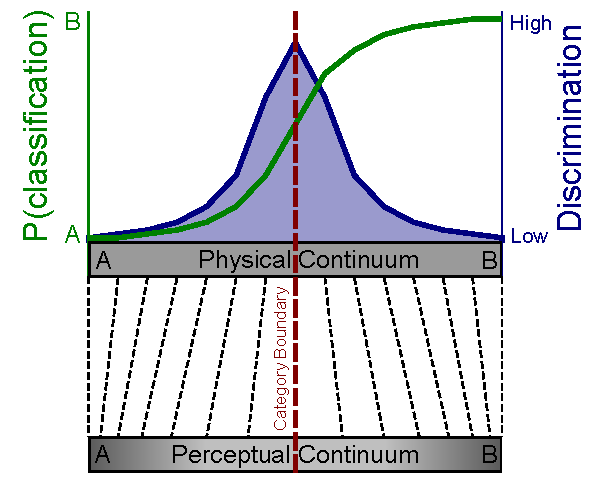
\includegraphics[width=0.75\textwidth]{figures/cp_def.pdf}
  \caption[A schematic of idealized categorical perception]
{\emph{A schematic of idealized categorical perception}. \emph{Top green}: The psychometric function or the probability of classifying a stimulus as A or B as you move along a physical continuum between A and B. The category boundary occurs at the vertical red dotted line and there is some amount of uncertainty near this boundary. The boundary is defined as the point of perceived equality or the stimuli location on the physical continuum where a participant is equally likely to classify the stimuli as A or B. \emph{Top Blue}: is the discrimination curve describing how well a participant can discriminate between nearby stimuli. \CP has been described as a peak in the discrimination curve near the category boundary. The lower axis indicates how the perceptual space is stretched compared to the physical continuum causing stimuli that are within category limits to be perceived as closer than stimuli that lie across category boundaries but are an equal distance apart.\index{cp}}
  \label{fig:cpdef}
\end{figure}

\section{What is required for \CP research?}

The fundamental difficulty with \CP research is that it generally occurs in the perception of a high dimensional space where naturally occurring ecologically relevant stimuli exist only on non-uniformly distributed sub-manifold of that space. In terms of auditory \CP in human speech, the high dimensional space is the space of all possible sounds that could possibly be heard, most of which would sound like random noise. The naturally occurring ecologically relevant stimuli are all the possible spoken sounds or phonemes that are useful for human speech production and comprehension, which exist in a much smaller lower-dimensional subset of all possible sounds. Even within this subset of sounds, not all possible phonemes are heard with equal probability, and this distributional information may begin to shape our perceptual systems even before birth.

Because of this, the majority of auditory \CP has focused on human speech sounds, predominantly English, leveraging our intuitions and years of linguistic modeling to identify the relevant dimensions where \CP occur. \CP work concerning animal vocalizations must first identify stimuli that are categorically perceived, a process that was very labor intensive \cite{nelson1989categorical,prather2009neural,lachlan2015context} before the development of more modern techniques \cite{sainburg2019parallels}. The variation within the songs of European starlings also makes this task easier because clustering song elements is more straightforward with more distinct clusters.

Furthermore, the identification of category boundaries is more difficult in non-human research than with human subjects. Since we can't provide instructions, we are forced to use multiple shaping or pre-training stages of operant behavioral conditioning. Also, if we permit a fully adaptive double staircase procedure, our subjects learn to exploit this and force the boundary all the way to one side or another. To solve this, we use a new staircase technique.

Last, but certainly not least, \CP requires the generation of a synthetic continuum between the categories or category exemplars. In human speech, the existence of speech synthesizers has made this task easy, at least in English. In Chinese for example, the technical difficulty in creating a Chinese-based synthetic continuum suitable for a \CP study has been proposed as a reason for the large number of papers focused on \CP in lexical tones in the Chinese language \cite{zhang2013categorical}. \CP research on animal vocalization has been limited to exploiting natural variation in recorded calls \cite{nelson1989categorical,prather2009neural,lachlan2015context} which invariably limits the sampling and control over the stimuli. It has also been shown that the quality of the speech synthesizer is correlated with how much \CP is observed\cite{van1999categorical}.

Thus the approach we present streamlines the following steps for \CP research in non-human vocalizations:
\begin{enumerate}
    \item Identification of relevant dimensions where \CP occurs
    \item Identification of categorical boundaries
    \item Generation of a synthetic continuum between the categories/ category exemplars.
\end{enumerate}

\section{History of Categorical Perception}

There is a long history of categorical perception research.
The invention of the formant speech synthesizer known as the Pattern Playback at Haskins Laboratories \cite{patternplayback} made the discovery of \CP possible.
The Pattern Playback was a machine that converted pictures of the acoustic patterns of speech in the form of a spectrogram into sound using light.

\CP was initially described as the absolute definition of completely quantal perception where subjects would be unable to discriminate differences to stimuli within a category, only noticing differences in stimuli that lies across category boundaries \cite{liberman1957discrimination, Studdert1970motor}. Although only ever described as an idealized case, this definition is far too restrictive and has been disproven many times; however, it has caused much criticism of the work done in the \CP field with critics calling for ``The end of categorical perception as we know it'' \cite{schouten2003end} etc.

Later work has instead demonstrated that with-category differences are discriminable \cite{pisoni1974reaction,carney1977noncategorical,massaro1983categorical} and meaningful \cite{miller1997internal,mcmurray2002gradient,mcmurray2008gradient}. Thus it seems there is just an increase in sensitivity to differences in stimuli that lie across category boundaries.

\CP first explored in 1957 concerning the discrimination of speech sounds within and across phenome boundaries \cite{liberman1957discrimination}.  In addition to dubbing the term ``Categorical Perception,'' Liberman suggested that \CP was unique to human speech, and furthermore, was what made human speech special. He also originally proposed the motor theory of speech perception \cite{liberman1967perception}.

Formerly thought to be peculiar to speech and color perception, \CP turns out to be far more general and may be a result of the way our neural circuits are wired to identify hierarchical patterns.

\CP also provides an intermediate explanation of equivalence classes which in turn form the basis of high-level symbolic thought and auditory \CP also forms the basis for human language.

Auditory \CP was previously thought to be strictly human trait possibly depending on special processing or that there might be some motor theory basis that could inform perception based on a motor production model. It is now thought to be a ubiquitous feature of all perceptual systems.

It has been shown in chinchilla \cite{kuhl1975speech} and later in macaques \cite{kuhl1983enhanced}, that animal models also have enhanced discriminability at human phonetic boundaries without a phylogenetic history of phenomic knowledge, either acoustic or articulatory.
These studies consist of playing human speech sounds to animals and behaviorally measuring if they place the same boundaries we do.
This has been used to argue that human languages may have adapted to use phenome category boundaries located in regions with intrinsically higher discriminability \cite{stevens1981constraints,goldstone2010categorical}

There also exists a host of research on \CP in non-human vocal communication sounds. These studies either use
natural variation in the vocalizations
artificially generated hand drawn spectrogram morphs.
These studies are only possible after considerable background work establishes the relevant categories, similar to the techniques originally used in humans to identify \CP.

Categorical boundary location preference has also been explored, mostly in the context of human speech. Early explanations included the motor theory of speech perception, which suggested that the explanation for \CP lay in the anatomy of speech production, specifically, physical differences during articulation \cite{liberman1967perception}. There have also been arguments made that a biological predisposition influenced the development of human languages pushing phenome boundaries to locations of increased sensitivity \cite{stevens1981constraints, goldstone2010categorical, halle1979some}

\section{Learned Categorical Perception}

However, we also know that the boundary location is experience dependent. Native language exposure can shift boundary locations. Also, a sound difference that crosses a boundary of a language is more discriminable to speakers of that language than to speakers of a language that doesn’t have a boundary in that location.

\comment{Lots more here about learning on \CP, also context dependency}

\section{Our Contribution}
We use machine learning techniques to approximate unsupervised statistical learning of the distribution of the set of natural motifs while compressing it into a lower dimensional representation. This allows us to generate a continuum of synthetic motifs that lie between exemplars.

These types of machine learning methods allow for the creation of synthetic continua between exemplars when trained upon a corpus of that stimuli type. This allows for the exploration of natural ecologically relevant animal communication signals as we have done here. It also would allow the exploration of categorical perception in non-English languages. For example, technical difficulty in creating the Chinese-based synthetic continuum suitable for a \CP study has been proposed as a reason for the large number of papers focused on \CP in lexical tones in the Chinese language \cite{zhang2013categorical}.

Furthermore, stimulus naturalness has been shown to be a factor determining the degree of categorical perception\cite{van1999categorical}, so as these machine learning techniques improve, we may be able to better explore the \CP phenomena.

Our method allows for the creation or discovery of boundaries of \CP in an unsupervised way in animal vocalizations and are thus more ecologically relevant and activate auditory regions that are specifically tuned to conspecific vocalizations.
\chapter{Categorical Perception}
\begin{flushright}
{\large Synthetic vocalizations reveal a shared perceptual space\\ predicted by relationships in neural population activity\\ shared across birds and recording sites}
\end{flushright}

\section{Abstract}
Parametrizing complex natural stimuli is a difficult and long-standing challenge. We used a generative deep convergent network to represent and parametrize a large corpus of song from European starlings, a songbird species, into a compressed low-dimensional space. We applied psychophysical methods to probe categorical perception of natural starling song syllables, which reveal a shared categorical perceptual space. Some categorical boundaries are sensitive to the category assignment of training syllables, indicating that the consensus is context dependent and that underlying dimensions of the space are not independent. We record simultaneous firing from populations of 10's of neurons in a secondary auditory cortical region of anesthesized starlings. By estimating how fast population level neural representation change with respect to the stimuli, we produce a measure along a path in stimuli space that is shared between birds and descriptive of the psychophysically determined parameters in other birds. Consistent with this, we predict the behavioral psychometric function along one dimension by fitting the behavior for other dimensions to the population level neural activity. Thus, knowing how the animal responds in one sub-region of the parametrized space informs responses in other sub-regions. Our results implicate the importance of experience in shaping shared perceptual boundaries among complex communication signals, and suggest the categorical representation of natural signals in secondary sensory cortices is distributed much more densely than predicted by traditional hierarchical object recognition models.

\section{Introduction}
\acf{CP} is the phenomenon where categories held by the observer, either learned or inherent, influence the observer's perception. This means that the perception of changes in the stimuli does not depend solely on the physical changes in the stimuli. Small changes in stimuli that move near or across category boundaries are very noticeable while more substantial changes in other regions may not be noticeable at all. This means that our perceptual system transforms relatively linear sensory signals into relatively nonlinear interval representations.

Experimentally we observe \CP as demonstrated in figure (\ref{fig:outline}A). For a defined physical continuum that moves between two (or more) categories, A and B, for example, we can experimentally ask a participant to classify the stimuli as belonging to category A or category B. This provides the sigmoid-shaped psychometric curve shown in green in figure (\ref{fig:outline}A) where the probability of classifying a stimulus as category B is high when the stimulus is near the B category and low when the stimulus is near the A category. Another \CP hallmark is a peak in the discrimination function near the boundary of two categories. This is tested by experimentally asking a participant to distinguish nearby stimuli on the physical continuum, and is shown in blue in figure (\ref{fig:outline}A). Thus, the physical continuum is perceived as being stretched near the category boundary and compressed within category limits.

The conventional view of the auditory object processing pathway (Ventral Auditory Pathway) is very similar to the visual object processing pathway (Ventral Visual Pathway). The ventral auditory pathway consists of the hierarchical processing of categorical information where neurons become increasingly sensitive to more complex stimuli and abstract information between the beginning stages and the latter stages. It is therefore theorized that as you move along the ventral auditory pathway, there is a progression of category information processing, where simpler receptive fields are combined to form more and more complex receptive fields encoding more and more complex features of the stimuli until you reach the auditory equivalent of a ``grandmother cell.'' Perhaps not quite as extreme as proposing the existence of the auditory equivalent of a ``grandmother cell,'' there are regions such as the superior temporal gyrus and sulcus which is categorically activated by speech sounds, relative to other sounds \cite{Binder2000, leaver2010cortical} and there are distinct regions of superior temporal gyrus and sulcus that are selectively activated by musical instruments sounds \cite{leaver2010cortical} and even tool sounds and birdsong \cite{doehrmann2008probing}.

European starlings ({\it Sturnus vulgaris}) are an excellent established model organism to study auditory processing and categorical perception. Like human speech, starling song is composed of learned, spectrally complex, temporally-patterned acoustic objects (called \textit{\textbf{motifs}}), that are produced in long, well-organized temporal sequences \cite{gentner2003neuronal}, and that function in a wide range of natural behaviors. As with other complex natural signals, our understanding of how birdsongs are represented in higher cortical regions, both benefits from and is hindered by the complex spectro-temporal character of these sounds. Multiple physiological studies have used conspecific vocalizations, and reveal a strong selectivity for songs that emerges across the auditory forebrain and strengthens from field L to \ac{NCM} and \ac{CM} \cite{gentner2003neuronal, gentner2004neural, thompson2010song, jeanne2011emergence}.

Starlings rely on object-level representations of motifs \cite{Meliza2010,gentner1998perceptual,Comins2013,comins2014auditory}, and the neural correlates of motif perception are localized in the regions of the auditory forebrain \emph{that are evolutionarily homologous to the mammalian auditory cortex\cite{wang2010laminar}}. The songbird auditory system follows the vertebrate plan\cite{Carr1992}. Field L2a is the primary telencephalic target of the auditory thalamus\cite{Karten1968}, and is the input layer for a columnar circuit spanning L1, L3, and \ac{CM}, anatomically\cite{Wang2010a,Jarvis2005}, genetically\cite{Dugas-Ford2012}, and functionally\cite{Calabrese2015} analogous to the mammalian auditory cortical micro-circuit. Field L sub-regions also project to the \ac{NCM}, a region that, along with the \ac{CLM}, shares reciprocal connections with the \ac{CMM}. Neurons in \ac{NCM} have been shown to have complex composite receptive fields\cite{kozlov2016central} that are reminiscent of the multidimensional receptive fields found in cat A1\cite{atencio2008cooperative}. Multidimensional receptive field characteristics can be reproduced by a \ac{DNN}\cite{kozlov2016central} trained to represent starling songs. Neurons throughout the avian cortex are selective for species-specific (conspecific) vocalizations\cite{Bonke1979,Leppelsack1976,Muller1985}, with selectivity increasing from Field L2, to L1 and L3\cite{Theunissen2004,Theunissen1998,Theunissen2000}, and again in \ac{NCM} and \ac{CM}\cite{Calabrese2015,Muller1985,Grace2003,Bonke1979,Leppelsack1976,gentner2003neuronal,Gentner2004,Thompson2010,Jeanne2011}. This is consistent with a functional hierarchy tuned to conspecific song\cite{Hsu2004,Woolley2005}, refined by experience\cite{gentner2003neuronal,Sockman2002,Sockman2005,Phan2006,Thompson2010,Jeanne2011}, with selectivity for acoustic features at multiple timescales increasing in a feed-forward manner\cite{Rose1988,Kaas2000,Binder2000,VanEssen1992}. Because of its compact organization, close relation to well-studied sensorimotor/vocal production structures, and the rich behavioral history of birdsong, the system is ideal for understanding the processing of natural acoustic communication signals.
Starlings respond to natural complex stimuli patterns such as the presence or absence of a center-embedded recursive structure\cite{gentner2006recursive,comins2014auditory,comins2014temporal}, a characteristic previously thought unique to human language (at least by Chomsky), allowing access to signals that would be invasive in humans, and cost prohibitive in non-human primates.

\subsection{The difficulties of using European Starlings}

However, the lack of parametric control over the complex acoustic features composing birdsongs (and other communication signals in other species) had rendered it difficult to more rigorously and extensively characterize both the information that these regions encode, and how this information is encoded. Ideally, we would like to parametrically control the complex natural stimuli to which high-order sensory regions are tuned, with the same precision and control that past studies have manipulated more simple stimuli like white noise and simple sine wave stimuli that can drive more primary sensory regions.

Furthermore, starlings are not among the most popular model organisms, so many of the off the shelf tools available for other model organisms haven't been established for the Starlings. This includes the genetic and viral tools as well as off the shelf hardware and tools.

Lastly, increased mobility (3-dimensional freedom and frequent backflips) makes recordings while behaving more difficult, even though there have been examples of it\cite{knudsen2013active,bluvas2013attention}.

\subsection{What is required for \CP research?}

The fundamental difficulty with \CP research is that it generally occurs in the perception of a high dimensional space where naturally occurring ecologically relevant stimuli exist only on non-uniformly distributed sub-manifold of that space. In terms of auditory \CP in human speech, the high dimensional space is the space of all possible sounds that could possibly be heard, most of which would sound like random noise. The naturally occurring ecologically relevant stimuli are all the possible spoken sounds or phonemes that are useful for human speech production and comprehension, which exist in a much smaller lower-dimensional subset of all possible sounds. Even within this subset of sounds, not all possible phonemes are heard with equal probability, and this distributional information may begin to shape our perceptual systems even before birth.

Because of this, the majority of auditory \CP has focused on human speech sounds, predominantly English, leveraging our intuitions and years of linguistic modeling to identify the relevant dimensions where \CP occur. \CP work concerning animal vocalizations must first identify stimuli that are categorically perceived, a process that was very labor intensive\cite{nelson1989categorical,prather2009neural,lachlan2015context} before the development of more modern techniques\cite{sainburg2019parallels}. The variation within the songs of European starlings also makes this task easier because clustering song elements is more straightforward with more distinct clusters.

Furthermore, the identification of category boundaries is more difficult in non-human research than with human subjects. Since we can't provide instructions, we are forced to use multiple shaping or pre-training stages of operant behavioral conditioning. Also, if we permit a fully adaptive double staircase procedure, our subjects learn to exploit this and force the boundary all the way to one side or another. To solve this, we use a new staircase technique.

Last, but certainly not least, \CP requires the generation of a synthetic continuum between the categories or category exemplars. In human speech, the existence of speech synthesizers has made this task easy, at least in English. In Chinese for example, the technical difficulty in creating a Chinese-based synthetic continuum suitable for a \CP study has been proposed as a reason for the large number of papers focused on \CP in lexical tones in the Chinese language\cite{zhang2013categorical}. \CP research on animal vocalization has been limited to exploiting natural variation in recorded calls\cite{nelson1989categorical,prather2009neural,lachlan2015context} which invariably limits the sampling and control over the stimuli. It has also been shown that the quality of the speech synthesizer is correlated with how much \CP is observed\cite{van1999categorical}.

Thus the approach we present streamlines the following steps for \CP research in non-human vocalizations:
\begin{enumerate}
    \item Identification of relevant dimensions where \CP occurs
    \item Identification of categorical boundaries
    \item Generation of a synthetic continuum between the categories/ category exemplars.
\end{enumerate}

\section{Results}
\begin{figure}[tp]
\caption[Task outline]{
\emph{Task outline}
(A) A schematic of idealized categorical perception. \emph{Top green}: The psychometric function or the probability of classifying a stimuli as A or B as you move along a physical continuum between A and B. The category boundary occurs at the vertical red dotted line and there is some amount of uncertainty near this boundary. The boundary is defined as the point of perceived equality or the stimuli location on the physical continuum where a participant is equally likely to classify the stimuli as A or B. \emph{Top Blue}: is the discrimination curve describing how well a participant can discriminate between nearby stimuli. \CP has been described as a peak in the discrimination curve near the category boundary. The lower axis indicates how the perceptual space is stretched compared to the physical continuum causing stimuli that are within category limits to be perceived as closer than stimuli that lie across category boundaries, but are an equal distance apart.
(B) A diagram of the operant behavioral apparatus which consists of response ports with IR beak detection sensors, a food hopper to provide access to a food reward, and a speaker hidden behind the panel to present auditory stimuli.
(C) A diagram of generating an interpolating morph using a \DBN autoencoder. A spectrogram representation of two 400 ms song motif, A and D, are fed into a compressive network to create a latent representation, $Z_A$and $Z_D$. We then linearly interpolate between $Z_A$and $Z_D$ to create $Z_{ADmorph}$ which we can use to reconstruct a spectrogram motif that lies between A and D. Three example morph interpolations are shown below in (E)
(D) Diagram of the behavioral task. Spectrograms of the initial 8 randomly chosen 400 ms long motifs, labeled A-H, and their reward associated responses. Once the performance on these 8 reached a sufficient stable level, interpolated morph motifs, indicated by the 16 connecting lines were probed using a ratcheting double staircase procedure to allow the birds to determine their own behavioral boundaries.The 3 example morph dimensions displayed to the left are highlighted in blue.
(E) Three example interpolated morph dimensions generated using the \DBN. 16 (of 128 used) example motifs for each morph dimension. Spectrogram representation with frequency on y-axis and time on the x-axis. Each motif is 400 ms long.
\index{outline}}
\end{figure}

\begin{figure}[tbp] 
\contcaption{\emph{Task outline} Continued from previous page.}
  \centering
  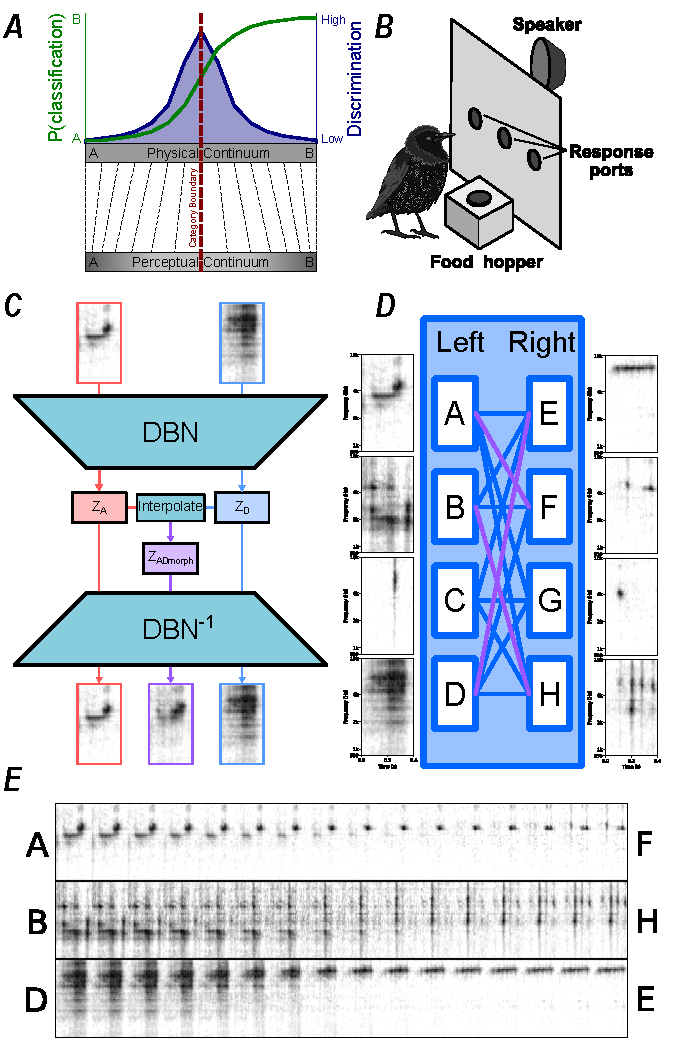
\includegraphics[width=114mm]{figures/fig01_task_outline.pdf}
  \label{fig:outline}
\end{figure}

\subsection{Generating smoothly varying morphs}

Using a large corpus of recorded starling song, a generative machine learning model is trained to non-linearly autoencode 400 mS motifs (song segments) of starling song in a low (64) dimensional latent space. The generative model attempts to model the distribution of song segments the model is trained on and as a result it tries to completely fill the latent space with projected representations due to an information bottleneck. The consequence of this is that for any point in the latent space, the spectrogram reconstruction of that point could lie within the actual distribution of starling song. Thus, the model can be used to interpolate between any two arbitrarily chosen starling motifs projected into the latent space to produce a smoothly varying continuum of morphed motifs that shift from one target motif to the other as outlined in \ref{fig:outline}(C). Instead of sounding like a simple linear crossfade between the two motifs, the network tries to produce a motif that could be in the distribution of recorded motifs, resulting in more realistic sounding motifs. Three examples of these smooth morphs are shown in \ref{fig:outline}(E) 

\subsection{Behavioral Measurement of Perceptual Space}

Using an operant behavioral apparatus diagrammed in \ref{fig:outline}(B), starlings are trained on a two alternative choice task where four arbitrarily chosen motifs (labeled A, B, C, and D) are associated with a left response and another four (E, F, G, and H), are associated with a right response as summarized in figure \ref{fig:outline}(D). After training to a stable performance criterion, the interpolated morph motifs generated by the \ac{DBN} are used to probe the bird's perception as each left-associated motif is transformed into each right-associated motif. We employed a ratcheting double staircase that \emph{allowed us to iteratively (and independently) estimate the categorical boundary along each of the 16 morph dimensions for each bird}. 

\subsection{Psychometric curves are conserved across subjects}

\begin{figure}[tp]
  \caption[Psychometric curves are conserved among different birds]{
  \emph{Psychometric curves are conserved among different birds}
(A)	Construction of a single psychometric curve: The x-axis represents presentations of stimuli that vary between motif A on the left and motif E on the right. The middle tick mark is the location of a stimuli that lies exactly between motif A and motif E (according to the \DBN). Thus the 3 tick marks indicate the location of stimuli that is (left) 75\% A, 25\% E, (middle) 50\% A, 50\% E, and (right) 25\% A, 75\% E. The y-axis is the probability of a right response (that has been operantly conditioned to be associated with motif E). The black dots represent the binary decision of the birds (responses are jittered to demonstrate relative density). All the responses ordered by morph position are binned into 16 equally sized bins and the 95\% confidence intervals of the mean estimates are plotted as vertical blue lines. The maximum-likelihood 4 parameter logistic fit of the probability of the bird responding right as a function of morph position between motif A and motif E, which we will call the psychometric curve, is plotted in blue.
(B)	Psychometric curve variation: The set of all 16 behaviorally determined psychometric curves for a single bird. Color indicates each of the 16 different morph dimensions.
(C-D)	Exemplar psychometric curves that are conserved between subjects: 2 of the 16 morph dimensions, (C) motif B to motif F and (D) motif A to motif H, are plotted for 4 different birds trained on the same categorization task. The full 16 dimensions are plotted in supplemental figure \ref{fig:psychometric-all}.
(E)	To measure how the B parameter (determines boundary sensitivity or slope at the boundary) of the psychometric curves is grouped we take the one-sided \KS metric between the distribution of pairwise distances between the B parameter of all psychometric curves, to the distribution of pairwise distances between the B parameter of psychometric curves from the same morph dimension (blue), and to the distribution of pairwise distances between the B parameter of psychometric curves from the same bird (red). The vertical blue line represents the \KS statistic between the distribution of pairwise distances between psychometric sensitivities that share the same morph dimension to that of all measured psychometric curves. The blue shaded cumulative survival curve is the distribution of expected \KS statistic values if we randomly split the psychometric curves into groups that share the same size as the morph dimension groups, or the null distribution as estimated by $2^{17}=131,072$ shuffles. Thus, the interception of the vertical blue line with the blue shaded cumulative survival curve provides an estimate of the likelihood that the psychometric sensitivities are as close to the psychometric sensitivities of other birds on the same morph dimension by chance, $p=3E-4$. We use an 8-way bonferroni correction to account for the 2 groupings and 4 parameters we test. * indicates $p<0.00625$, **, $p<0.00125$, and ***, $p<0.000125$. The vertical red line is the \KS statistic between the distribution of pairwise distances between psychometric sensitivities from the same bird to the distribution of pairwise distances between all psychometric sensitivities. Its corresponding shuffled null distribution is plotted as the red shaded region providing an estimate of $p=0.044$. Together, this indicates that psychometric sensitivities are closer than would be expected by chance when grouped by morph dimension, but not when grouped by bird. (continued on following page)
\index{conserved}}
\end{figure}


\begin{figure}[tbp] 
  \contcaption{
  \emph{Psychometric curves are conserved among different birds} Continued from previous page.
  (F)	The corresponding figure for the M parameter (boundary location). This shows that the likelihood that the psychometric boundaries are as close to the psychometric boundaries of other birds on the same morph dimension by chance (blue), $p<8E-6$ because never once in all the $2^{17}$ shuffles, was the KS statistic as great as the value measured. When distances between psychometric boundaries within a single bird are considered (red), $p=0.041$. This indicates that psychometric boundaries are also closer than would be expected by chance when grouped by morph dimension, but not when grouped by bird. Parameters A and K, the maximum accuracy achieved near each endpoint, are plotted in supplemental figure \ref{fig:AKconserved} and show the opposite trend.
}
  \centering
  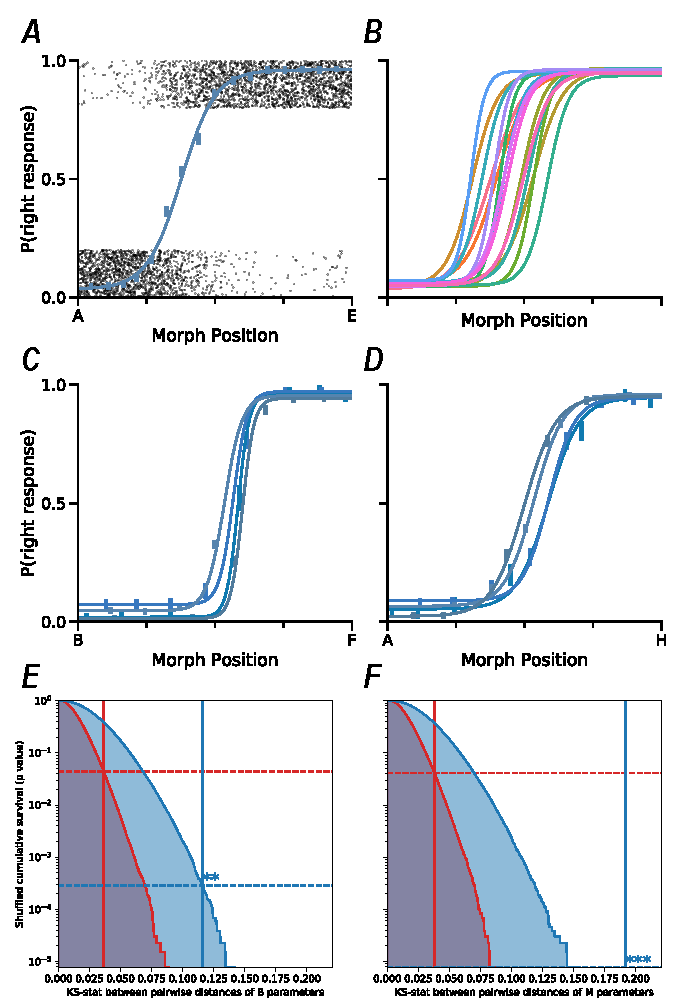
\includegraphics[width=114mm]{figures/fig02_conserved.pdf}
  \label{fig:conserved}
\end{figure}

This provides independent binary behavioral responses along each of the 16 possible dimensions interpolating from each of the 4 left associated motifs to each of the right associated motifs.

We fit a \textit{\textbf{psychometric curve}} of the form $P(R) = A + \frac{K - A}{1 + e^{-B(x-M)}}$ using maximum log likelihood for each of the 16 morph dimensions. $A$ and $K$ determine the maximum accuracy achieved near each endpoint. $M$ determines the boundary location or the point of subjective equality between each of the endpoints. $B$ determines boundary sensitivity or slope at the boundary.

A psychometric curve is fit to these behavioral responses and figure \ref{fig:conserved}(A) demonstrates how well a four parameter psychometric curve fits the average response along a single example dimension. We measure 16 of these curves for each bird.

In all cases, birds show very clear categorical perception as evidenced by the steepness each psychometric function regardless of bird or motif dimension. Comparing the psychometric curves within a single bird across all 16 motif-to-motif dimensions reveals a large amount of variation in the point of subjective equality (the category boundary) and in how sensitive the bird is to stimulus changes across the boundary (Fig. \ref{fig:conserved}(B)). This variability across dimensions is presumably a result of the non-linear nature of the \ac{DBN} song compression and morphing. Thus, we can conclude that \emph{the features the DBN uses to represent the motifs are perceptually relevant to the starlings}, and that the starlings are differentially sensitive to variation along these different feature dimensions.

Despite the significant variability within a single bird across multiple morph dimensions, we observed a remarkable degree of consensus between birds.  This included strong agreement in where each bird placed the category boundary on a given dimension, and in the sensitivity of all birds to changes along a given stimulus dimension (slope of psychometric function). Figure \ref{fig:conserved}(C-D) gives an example of the typical agreement between birds, where two of the 16 morph dimensions are plotted for 4 different birds.

Psychometric curves for four starlings, over several months of training, are highly conserved between individuals, suggesting a shared perceptual space. The y-axis shows the probability of a right response to a stimulus morphed continuously between, for example on the left, motif B (reinforced as left) and motif F (reinforced as right). The x-axis is the morph position between the left associated motif to the right associated motif.

$A$ and $K$, the left and right scaling parameters are statistically closer than would be expected when compared across all morphs within a single bird indicating that they are bird specific parameters as demonstrated by supplementary figure \ref{fig:AKconserved}. This makes sense because they correspond to the bird's absolute performance on the left and right endpoints. Figure \ref{fig:conserved}(E-F) also show that $M$, the category boundary and $B$, the sensitivity are conserved within the same morph dimension across different birds, but not within a single bird. This indicates the existence of a shared perceptual space of these synthetic natural-like sounds in these wild caught birds. 

\subsection{Different training context sometimes results in reliable shifts in the psychometric curves}

\begin{figure}[tbp] 
  \centering
  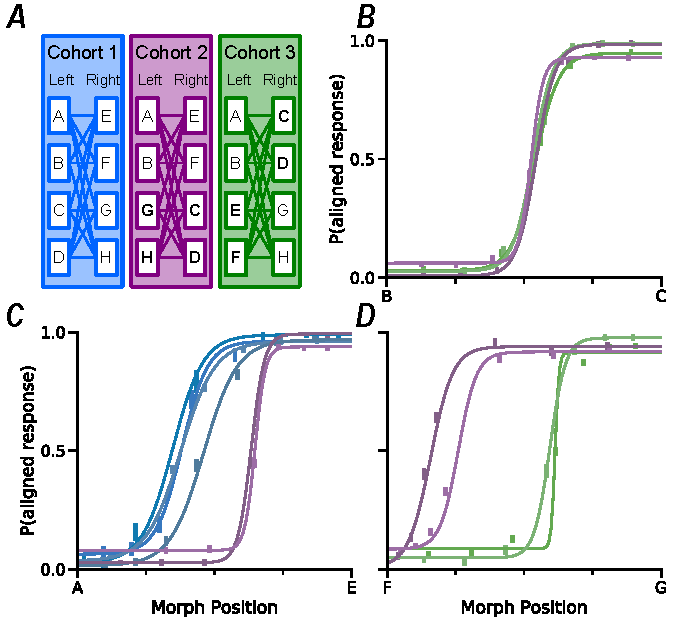
\includegraphics[width=114mm]{figures/fig03_shift.pdf}
  \caption[Different training context sometimes results in reliable shifts in the psychometric curves]
{
(A)	Diagram of alternative training contexts. Task structure remains the same in each cohort, but some motif category assignments change. Category assignment differences from Cohort 1 are bolded in Cohort 2 and 3. This allows a subset of the morph dimensions to be compared across training on different category permutations. Colors correspond to colors used in adjacent plots.
(B-D)	Exemplar psychometric curves from subjects trained on different category permutations. 
(B)	On most dimensions the boundary is conserved as if the training was the same as shown in the psychometric curves from these 4 birds, 2 from each of cohort 2 and 3 along the morph dimension between motif B and motif C. 
(C-D)	However, on some of the dimensions, such as A to E (left) and F to G (right), the behaviorally measured boundaries depend on the initial categorical assignment.  When there is a difference, the boundaries are still conserved within cohorts.
\index{shift}}
  \label{fig:shift}
\end{figure}

The shared perceptual space for motif categorization may result from either common training and experience, idiosyncrasies of the compressive network transformation, or some combination of the two. To test for this, we permuted the initial motif category assignments for a subset of birds. Instead of associating motifs A, B, C and D with left responses and motifs E, F, G, and H with right responses, a new cohort of birds learned, for example, to associate motifs A, B, E, and F with left responses and motifs C, D, G, and H with right responses. The category assignments for the three different cohorts are shown in figure \ref{fig:shift}(A). Thus, a subset of the 16 interpolating morph dimensions between left and right associated motifs is shared with the original cohort's interpolating morph dimensions. Comparing these shared boundaries demonstrates that on some of the interpolated morph dimensions, both cohorts of birds place the boundaries in same location as shown in figure \ref{fig:shift}(B) while in other interpolating morph dimensions each cohort has a separate boundary (but consistent within that cohort), as shown in figures \ref{fig:shift}(C-D). The boundaries that are preserved across motif category permutation indicate that these dimensions are independent from the other dimensions, however, the boundaries that are shifted as a result of the motif category permutation indicate an interaction between the interpolated morph dimensions. This is unexpected, especially if one considers that in the latent space of the DBN there is minimal collinearity and no discernable structure between any of the 8 motifs used.


\subsection{Electrophysiological Recordings}

To explore the neural underpinnings of categorical perception we record from secondary auditory regions of anesthetized starlings and present the generated motifs. We record from a total of 2019 neurons in 47 recorded population sites in 8 different starlings, 4 having been trained on the task, 4 naive, never having heard the stimuli before. We use a 32 channel silicon electrode and stereotaxically target \ac{CMM} and \ac{CLM} as described in the methods and shown in figure \ref{fig}. We sort the data using MountainSort\cite{mountainsort}. 

\subsection{Single neurons have reliable temporally precise responses}

\begin{figure}[tp]
 \caption[Single neurons have reliable temporally precise responses]{
 \emph{Single neurons have reliable temporally precise responses}
(A)	Spectrogram representations of example stimuli presented to the anesthetized starlings of four example motifs presented, motifs A, B, F, and H.
(B) The equivalent audio waveform pressure representations. Black lines mark the start and end of the auditory stimuli.
(C) The raster plots of a single neuron for 240 presentations of each of these stimuli. Vertical marks are plotted at each time point of the occurrence of a spike in the 400 ms stimuli. The y-axis denotes the stimuli presentation. Black lines mark the start and end of the auditory stimuli.
(D) Average Gaussian convolved spike train representation in black. We convolve each individual trial with a Gaussian with $\sigma=10ms$ to get an instantaneous estimate of spike firing rate. These are plotted faintly to demonstrate trial to trial reliability and variance of this representation. The average of these 240 faint lines is plotted in black for each of these stimuli.
(E) Heatmap representation of the above representation to be used below. Lighter represents higher estimated instantaneous firing rate. These plots are all normalized to the max firing rate. The colored outlines indicate where the data is repeated below.
(F) Variation of the average Gaussian convolved single neuron’s representation across morph dimensions. Smoothly interpolated using triangulation for surface estimation. Morph position is plotted on the Y axis as the motif presented goes from motif A (highlighted in blue as a band along the bottom) to C (along the top) for example in the top left subplot. Time (during the stimuli presentation) is plotted on the X-axis. The representations of motif F (red) and motif H (Magenta) are diagrammed to demonstrate how the representation is using the average response of this neuron as the top row in the right two subplots in the top row of this representation. Other colors outline other areas that include the averaged representations from figure E.  Not all morph positions were presented the same number of times so confidence (not represented) varies along morph position axis.
\index{single}}
\end{figure}

\begin{figure}[tbp] 
\contcaption{\emph{Single neurons have reliable temporally precise responses} Continued from previous page.}
  \centering
  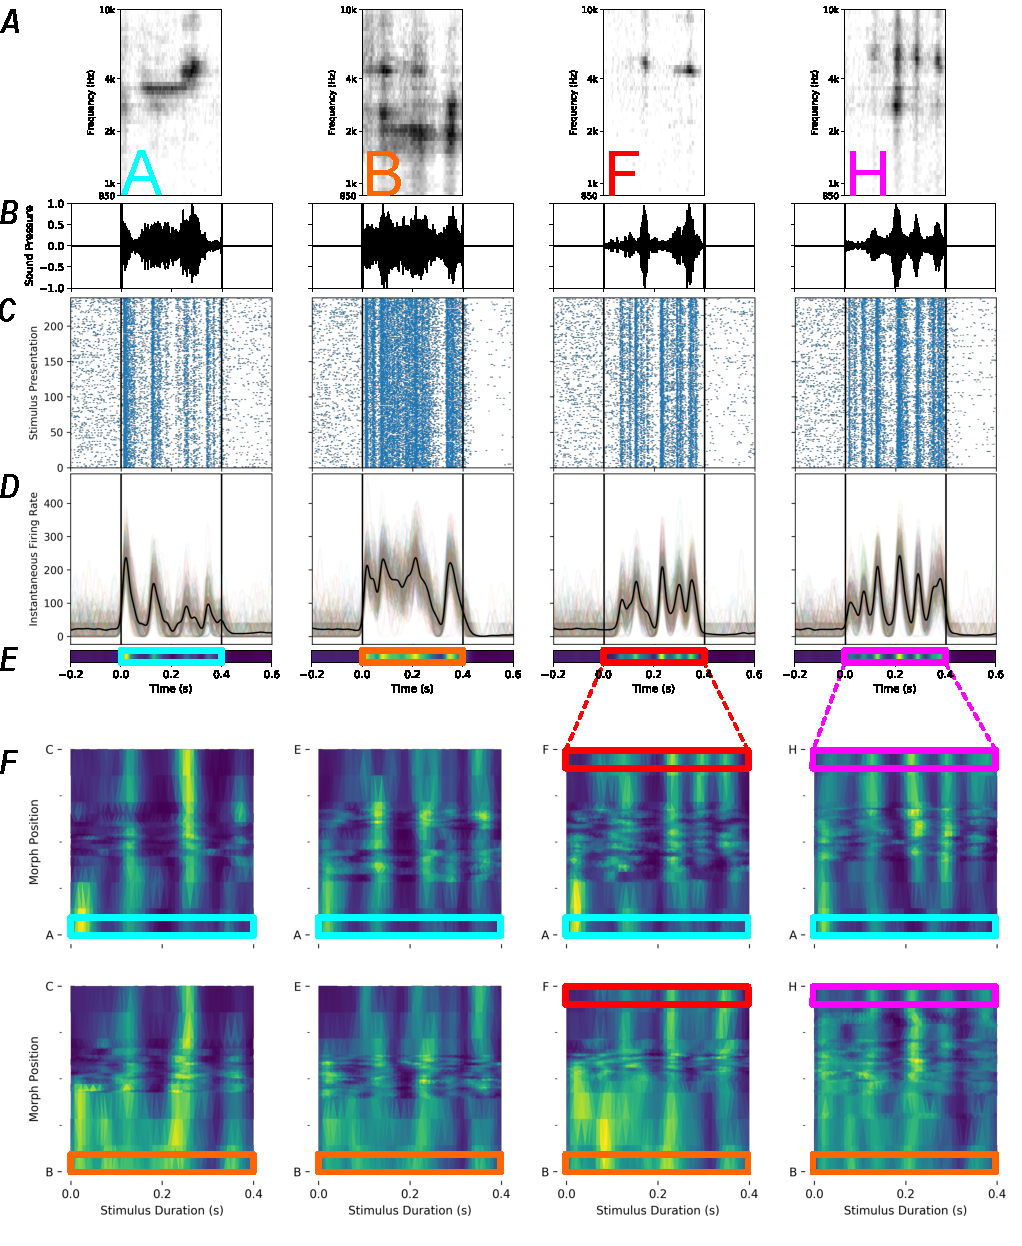
\includegraphics[width=\textwidth]{figures/fig05_single.pdf}
  \label{fig:single}
\end{figure}



We find the units are extremely time-locked and stimuli specific as demonstrated by figure \ref{fig:single}. Because of this we choose to include time in our neural representation by convolving the spike train with a Gaussian($\sigma = \SI{10}{ms}$). This provides us with a continuous estimate of firing rate through time for each trial for every unit. If we look at the average of this representation as we move along a morph dimension we find that there is a large amount of variation in how the units respond. Some units respond very smoothly to changes along a morph dimension, whereas others are quite categorical.

\begin{figure}[tbp] 
  \centering
  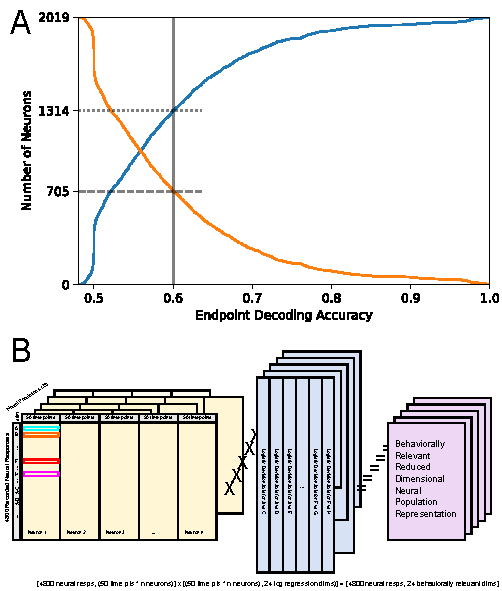
\includegraphics[width=114mm]{figures/fig06_neural_rep.pdf}
  \caption[Behaviorally relevant neural representation]
{
(A) The cumulative (blue) and survival (orange) curves for the distribution of units’ average accuracy on decoding pairs of the endpoint template motifs. The 0.6 accuracy cutoff was chosen mainly for computational tractability reasons. Subsequent analysis only includes activity of the 705 “behaviorally relevant neurons” with an average accuracy above 0.6. The 1314 neurons with average endpoint decoding accuracy below 0.6 were ignored by subsequent analysis.
(B) Diagram of the construction of the behaviorally relevant reduced dimensional neural population representation. We take the recorded neural representations from a population of “behaviorally relevant neurons”, sampled at 50 time points and concatenated to form a neural representation. We take the logistic decision axis for a logistic regression trained on the endpoints of the 24 morph dimensions to form the columns of a projection matrix which projects the neural population representation into 24 behaviorally relevant dimensions. The colored boxes correspond to the data which would be averaged to form the representations in the previous figure \ref{fig:single}. This behaviorally relevant neural representations are then used as the input to predict the Thielk curves (figure \ref{fig:derivative}) and and to predict the behavioral responses (figure \ref{fig:neurometric}). 
\index{neural_rep}}
  \label{fig:neural_rep}
\end{figure}

We restrict our analysis to units that are able to correctly identify the identity of our eight template motifs (averaged in a pairwise fashion so that 50\% is chance) more than 60\% of the time. This leaves 705 remaining "behaviorally relevant" units as seen in figure \ref{fig:neural_rep}.

\subsection{The \Thielk Curve}

\begin{figure}[tbp] 
  \centering
  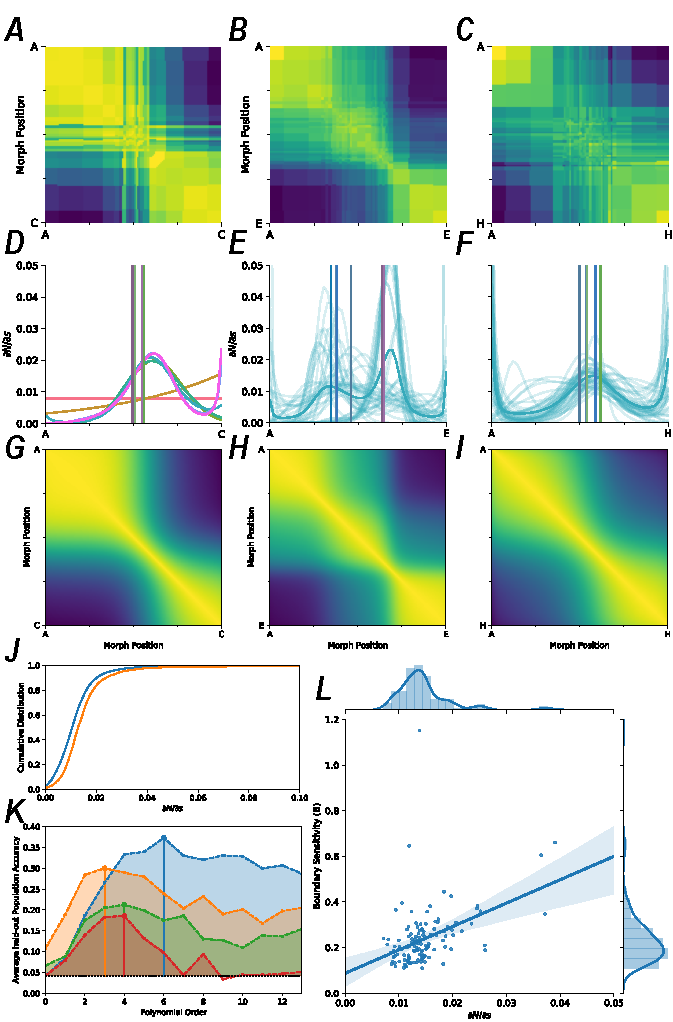
\includegraphics[width=114mm]{figures/fig07_derivative.pdf}
  \caption[The Thielk curve captures how neural representation changes as we move along a morph dimension]
{(continued on following page.)
\index{derivative}}
  \label{fig:derivative}
\end{figure}

\begin{figure}[tp]
  \contcaption{
(A)	The cross correlation matrix for a single recording on the morph dimension from motif A to motif C. Average cosine distance in the task relevant neural representation subspace between pairs of morph positions are initially calculated. These values are then upsampled to the full 128 pixel grid using nearest neighbor interpolation.
(B-C)	Average cross correlation matrix for all recordings (using the final stimuli set) for morph dimensions A to E and A to H.
(D)	Using a polynomial of order 0 through 6 to estimate the Thielk curve for a single recording and morph dimension, A to C (same as above).
Vertical lines represent the behaviorally determined psychometric boundaries for all birds tested across this morph dimension. The horizontal pink line is the 0th order fit, the exponential gold line is the 1st order fit.
(E-F)	4th order mean Thielk curves across all recordings on morph dimension AE (E) and AH (F). Individual 4th order Thielk curves for each recorded population are faintly plotted to show variance. Vertical lines represent the behaviorally determined psychometric boundaries for all birds tested across this morph dimension.
(G)	Cross correlation matrix reconstructed from the 4th order Thielk curve for the same recording used in (A) and (D).
(H-I)	Average reconstructed cross correlation matrix from all 4th order Thielk curves on AE (H) and AH (I)
(J)	Cumulative distributions of the value of the 4th order Thielk curve at psychometric boundary locations of the same dimension vs different dimensions as a control. A one-sided KS test provides a P value of $p=1.47E-121$
(K)	Average accuracy of predicting the morph dimension of a Thielk curve from a held out recorded neural population as we increase the order of the polynomial. The green and orange curves use the optimized polynomial coefficients to predict the morph dimension label. The red and blue curves use the normalized Thielk curve evaluated at 50 evenly spaced points along the morph dimension. The red and green curves use a multinomial logistic regression as the classification model. The orange and blue curves use XGBoost as the classification model. The vertical lines highlight the maximum average held-out prediction accuracy achieved by each method. Chance performance ($1/24$) plotted as a horizontal dotted line.
(L)	Correlation between the boundary sensitivity parameter (B) of the psychometric curve and the value of the 4th order Thielk curve for the given boundary location. Plotted above and to the right are the projected histograms and associated kernel density estimate of the distribution. Plotted as a line is the regression between these two variables with 1000 fold bootstrapped 95\% confidence interval plotted as a shaded region around the regression.
}
\end{figure}

We are interested in the brain's ability to discriminate changes along our morph dimension. We use distance in our neural representation to approximate the brain's ability to discriminate. 

We pose the following regression problem by defining the \Thielk curve:
Given a stimuli representation space $S$ containing $\{s_i\}$ that lie along a 1D path $s$ and a neural representation space $N$ for a given recorded neural population where we have samples of noisy projection, through a brain, of examples of $s_i$ into $N$, which we will call $\mathcal{B}(s_i):s_i \to N$.
We would like to define the following curve as $T(s_i)=\frac{\partial N}{\partial s} (s_i): s_i \in s$, such that for a pair of presented stimuli, $s_i$ and $s_j$, and a distance, $y=|\mathcal{B}(s_i) - \mathcal{B}(s_j)|$ in neural representation space between these to presentations, $y = \int_{s_i}^{s_j}T(s)ds + \epsilon$ . This assumes that the neural representation of these stimuli smoothly vary (up to some noise) as I move along the morph dimension. We then perform the regression to minimize the \MSE of $\epsilon$ for all pairs of stimuli presented on a single morph dimension.

The \Thielk curve measures how fast the neural representation changes as we move along a path in stimuli space. 

If we consider how the \Thielk curve is related to the cross correlation matrices plotted in figure \ref{fig:derivative}(A-C), it is a function defined along the diagonal and the value of each $i,j$ is the distance $y$ fit by the integral of the function from $(i,i)$ to $(j, j)$. Figure \ref{fig:derivative}(G-I) show how much of the structure in the cross correlation matrices in (A-C) are described by the \Thielk curves in (D-F)

We would like the \Thielk curve $T(s_i)$ to have the following properties: 1. Strictly positive. 2. Smooth over the range $D$.
To keep the function positive I have used $T(s_i)=e^{f(x)}$ and to keep it smooth I have used $f(x)$ as a polynomial of varying orders.
Several other parameterizations have been explored but they provided qualitatively similar results and took significantly longer to fit.

The polynomial parameterization and $s_i$ sampling makes the \Thielk curve highly susceptible to Runge's phenomenon near the ends of our morph dimension, especially for higher order polynomials. Therefore we do not interpret any spikes near the endpoints of our morph dimension as being meaningful.

Ignoring 0th and 1st order polynomial fits, higher order fits seem to all robustly fit the same curve shape as seen in figure \ref{fig:derivative}(D) with a peak near the behaviorally determined psychometric boundaries from other birds. This means that the neural representation was changing the fastest near the location on the morph dimension that other birds choose to place their boundary. This is less surprising when we see figure \ref{fig:derivative}(E-F) and see that the shape of the 4th order \Thielk curve is fairly similar for every single neural population recorded. Thus the \Thielk curve is a fairly recording invariant measure of changes in the neural representation. To statistically test this we try to predict the dimension a \Thielk curve describes without seeing any other data from a recording in figure \ref{fig:derivative}(K). We use two different prediction models and two different representations of the \Thielk curve and for each test our accuracy is much than the chance value of $1/24$. Each method-representation pair achieved max performance on held out populations using a polynomial order near a 4th order polynomial, which further reinforces are decision to use a 4th order polynomial fit. 

Lastly, if we consider the morph dimension from motif A to motif E (column BEH) where we observe a shift in the psychometric boundary between cohort 1 and 2, we see that many of the individual population \Thielk curves have two peaks, and there is certainly two peaks in the average \Thielk curve which correspond to the two locations of the psychometric boundaries.

If we compare the distribution of the value of the normalized \Thielk curve at the psychometric boundary location for psychometric curves on the same morph dimension to the values for different morph dimension in figure \ref{fig:derivative}(J), we see a clear shift in the distribution and a 1-sided \KS test confirms this with a p-value of $p=1.47E-121$ indicating that it is very unlikely that morph dimensions boundaries do not occur at locations on the morph dimension with higher \Thielk values than would be expected by chance.

Lastly, we use the natural variation in boundary location to test if greater \Thielk values are correlated with greater boundary sensitivity (B) in the measured psychometric curves. The relationship in the average \Thielk value of the psychometric boundary location to the boundary sensitivity (B) parameter has a Pearson's R correlation value of 0.42 which means we have a $p=6.5E-7$ that there is no correlation between these two variables.

\subsection{Predicting psychometric curves from neural population activity}
\begin{figure}[tbp] 
  \centering
  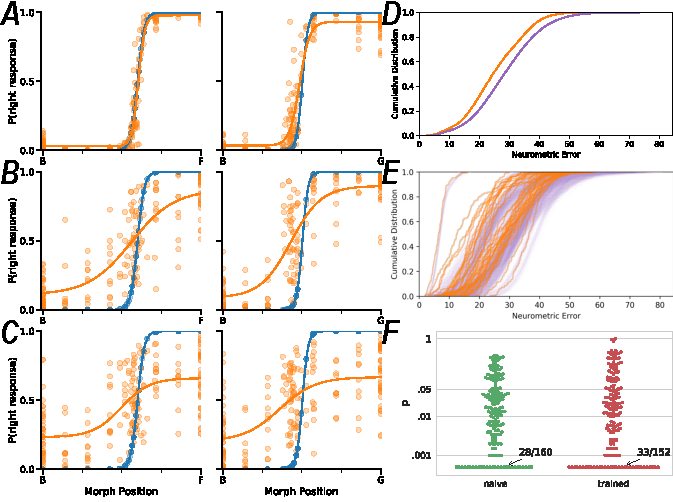
\includegraphics[width=114mm]{figures/fig08_neurometric.pdf}
  \caption[Predicting psychometric curves from neural population activity]
{
(A-C)   Predictions of behavioral psychometric curves for two morph dimensions, left: B to F, right:B to G, for the same behavioral bird, using three different recorded neural populations of differing quality. (A) shows an excellent fit, (B) shows a good fit, and (C) shows a fair fit for these two morph dimensions. Plotted in blue is the behavioral target, and plotted in orange are the held out predictions from a logistic regression trained on the other $15/16$ morph dimensions. The orange dots are the predicted probability of each stimuli presentation and the orange line is a 4 parameter logistic curve fit using \MSE to the probabilities. Some populations (A) do a lot better job at predicting the psychometric curves than others (C).
(D) Cumulative Distribution of the \MSE for neural predictions of the psychometric functions in orange and the cumulative distribution of the \MSE for neural predictions of shuffled psychometric functions in purple. This is the complete cumulative distribution for the \MSE for each of the 16 dimensions, for predictions against the psychometric curves of each behavioral bird (8), for all recorded neural populations (39).
(E) Same as (D) except plotted individually for each neural population in orange, and individually for each of 64 shuffles in purple.
(F) Shuffling each population against the behavioral curves 2048 times and comparing the \KS metric between the distributions allows us to estimate the p values for each neural population. Overall we find most population fits to perform better than would be expected by chance. Furthermore, if we split the recorded populations depending on whether they were from birds trained on this task or naive (never having heard the stimuli before) we find no difference in the distribution of p values. That is to say that a \KS test between the distribution of p values obtained for trained birds against the distribution of p values obtained for naive birds fails to reject the null hypothesis with a p value of $p=0.565$.
\index{neurometric}}
  \label{fig:neurometric}
\end{figure}

Using a hold-one-dimension-out cross validation strategy, we predicted the behavioral psychometric functions from the neural population representations. The behavioral response is fit given the neural representation of stimuli presented from 15 of the 16 interpolated morph dimensions and then the response is predicted on the neural responses of the remaining dimension. For computational tractability we used the behaviorally relevant reduced dimensional neural population representation described in figure \ref{fig:neural_rep}(B). The mean squared error for each held out dimension are combined to provide 16 performances for each neural recording (39?) for each set of behaviorally determined psychometric fits (8). We create a null distribution by shuffling the labels of the morph dimensions 2048 times and measuring the KS distance to distribution of 16 dimension performances by 8 behavioral bird's psychometric functions. Overall we find the fits are significantly better than would we expected by chance. Furthermore, if we compare the distribution of p values for recordings from untrained naive birds against the recordings of the birds that had been behaviorally trained we find that there's no difference between how well the neural representation of naive birds or trained birds can predict the location of the boundary or the sensitivity to changes near the boundary. That is not to say that there is no difference between the population representation in trained or untrained birds, or that more information about boundary location isn't encoded elsewhere in the brain, but that the information that allows generalization of categorical boundary parameters to other morph dimensions is equally present in both trained and untrained birds.

\section{Discussion}
To the best of our knowledge, this is the first single-unit level study where a vast (and arbitrarily chosen) selection of a species own vocal communication signals are used to understand categorization. Generalization in either response domain (behavioral or neural) was measured, and the only study where cross-domain (from neural to behavioral) generalization is shown.

Our results overcome a long-standing impediment to understanding the perception of natural communication signals. We demonstrate a method for parametrizing complex stimuli and generating \emph{smoothly varying morphs between these stimuli}, as well as how to use these morphs to explore the perceptual basis, behaviorally and neurally, of the natural stimulus space. To our knowledge, this marks one of the first naturalistic parametric explorations of non-human auditory communication signals. Our characterization of the perception of this space and its neurological underpinnings, reveals remarkable behavioral consensus between animals for categorical boundaries and a broadly distributed encoding strategy for categorical stimulus information at the neural population level.  

The observed shift in psychometric boundaries between cohorts was difficult to statistically explore because they only occurred in three of the 24 of the morph dimensions measured between the three cohorts. These shifts may indicate that depending on initial training conditions; birds may end up using different stimuli features to perform the classification or that discrimination along certain features may be altered by learning.

The work demonstrates the existence of a shared perceptual space, common across individuals, in which perceived categorical boundaries cluster at consensus locations.  This kind of consensus is a pre-requisite to functional communication systems that use discrete signals.  Furthermore, the 16 interpolating morph dimensions used in this study are not independent, nor are they a simple linear function of the endpoints, independent of the structure of the network space. If the latter were true, then all (or none) of the boundaries would shift when the endpoints were permuted. Instead, because only some of the dimensions are affected by permutation of the initial categories, not all the dimensions are independent, and the relationships between them are likely complex. Moreover, because there are dimensions that are not changed by the permutation of the initial categories, the decision boundaries learned by birds cannot rely on simple separation of the initial template motifs (as are seen in algorithms such as support vector machines or equivalent). Understanding where these boundaries fall likely requires knowledge of how natural stimuli is distributed in the latent space of the network, and the underlying geometry in which the latent manifold is embedded. Additional work is needed in these areas \cite{sainburg2019parallels}.

The field of machine learning is rapidly evolving, and there are several possible improvements to the processing and methodology. However, this work mainly demonstrates the usefulness of these kinds of techniques for understanding the perception of complex natural communication signals. In addition to changes in network architecture, newer implementations of spectrogram inversion would improve stimulus generation and are currently being tested and developed. In our experiment, however, different initializations of the spectrogram inversion process revealed that neurons in \ac{CM} are sensitive to these small physical differences in physical stimuli that are imperceptible to human ears.

One compelling result is that the behavior generalizes across this stimulus space, such that that knowing how perception acts in one sub-region can inform behavioral responses in other sub-regions. This category generalization also deserves further study.

Finally, the fact that categorical behavioral responses can be decoded from a randomly selected set of 10s of neurons contributes to a growing body of work \cite{jeanne2011emergence,kozlov2016central} that opposes the strongest version of sparse hierarchical models of perception, where neurons with simpler receptive fields converge onto neurons with more complex receptive fields until a complex percept, like Jennifer Aniston emerges \cite{quiroga2005invariant}. Under this model, decoding a categorical behavioral measure (as we show here) is only possible by matching the right stimuli to the right subset of neurons. Thus, our results imply that \emph{the representation of these secondary auditory regions is much more distributed than would be predicted by a model where increasingly complex features are encoded exclusively by single neurons}.

Using A DBN as a generative model of birdsong is another limitation of this work due to the amount of recent progress in machine learning. In particular, we recommend using \cite{GAIA} for these techniques as it can produce much more realistic sounding birdsong and is explicitly constructed such that the stimuli space is convex and interpolations between exemplars are realistic. There also exist a variety of other methods\cite{STRAIGHT, waveglow} that could be used to interpolate the songs.

Another possible limitation of these results is the anesthetized recording prep that was used. These measurements might not necessarily reflect the actual awake representations and especially attentional modulation, but certainly measure the functional tendencies of the network representation \cite{bluvas2013attention,knudsen2013active}. Additionally, this doesn't change our interpretation, which is based on the fact that we can predict categorical boundary parameters and not precisely what representation we are using to make the prediction.

While regions of the auditory forebrain are homologous to mammalian auditory cortex \cite{wang2010laminar}, there are significant structural differences. Thus, while solutions to the categorical perception of complex auditory stimuli used by birds aren't necessarily the same as those in our own, they do provide another example of a neural system capable of solving problems (recognizing complex hierarchical features and recursive grammars) previously thought to be strictly within human capacity. Thus, while it might not allow exploration of the neural circuitry we use, this line of work can perhaps indicate what kinds of circuit patterns and architectures could be useful in a system that needs this capacity.

\section{Methods}
\subsection{Contact for Reagent and Resource Sharing}
Further information and requests for resources and reagents should be directed to and will be fulfilled by the Lead Contact, Marvin Thielk (Marvin.Thielk@gmail.com).

\subsection{Experimental Model and Subject Details}
\subsubsection{European Starlings}
European starlings that have been wild-caught in southern California will serve as the experimental subjects. All subjects have full adult plumage when acquired, indicating they were at least one year old. Otherwise, I do not control for age or sex of the subjects. Subjects are housed in a large mixed sex, conspecific aviary with \textit{ad libitum} access to food and water from the time of capture until being moved into the testing chamber. The photoperiod in the aviary and testing chambers followed the seasonal variation in local sunrise and sunset times.

\subsection{Method Details}

\subsubsection{\ac{DBN} latent space morphs}
Using a large corpus of recorded starling song, a compressive \ac{DBN} \cite{hinton2006reducing} is trained to autoencode 400 mS sections of starling song. The Analysis \& Resynthesis Sound Spectrograph (ARSS) package was used to generate the spectrograms and perform the spectrogram inversion. We used >>>PARAMETERS<<<. We created a dataset of XXXXXXX samples of (possibly overlapping) 400 mS long spectrogram slices of size XXxXX = 7040 dimensions. We found that contrast normalizing the spectrogram using a logistic XXXXX on the outputs of the ARSS generated spectrograms. We tested several several layer size configurations and settled on a network with 5 encoding fully-connected hidden layers of sizes 1024, 512, 256, 128, and 64, which is then decoded back into 128, 256, 512, 1024, and finally back into the 7040 dimensional spectrogram space. The network is trained in a greedy layerwise fashion where the first layer is trained, then fixed, then the next layer is trained with the previous layers fixed, and so on until all layers are trained. Once the network has been trained, we can project a 400 mS motif, $A$, into the latent space, which we'll refer to as $Z_A = DBN(A)$, and then reconstruct the original spectrogram with the decoder network, $DBN^{-1}(DBN(A))$. In fact, the contrastive divergence learning algorithm used by the network tries to minimize the reconstruction error, $|A - DBN^{-1}(DBN(A))|$. We can also linearly interpolate between latent space representations of two motifs, $A$ and $D$, to generate a smoothly varying path in spectrogram space that morphs between $A$ and $D$. $\text{morph}(A, D, \tau) = DBN^{-1}(\tau DBN(A) + (1 - \tau) DBN(D)) | \tau \in [0, 1]$. For the experimental morphs I used $\tau \in \{ i/127\ |\ i \in [0, 127] \cap \mathbb{N}\}$. This process is diagrammed in \ref{fig:outline}(C)

\subsubsection{Operant panels}
Our testing boxes are acoustically isolated chambers containing a panel, shown in \ref{fig:outline}(B), with three response ports. I use PyOperant, an open sourced python package we have developed in the Gentner Lab, to reward the birds by raising a hopper of food to reinforce correct responses. Acoustic stimuli is delivered through a small full-range audio speaker mounted behind the panel and out of the subject's view. Water is unrestricted.

\subsubsection{Shaping}
I have coded an approximately unsupervised automated procedure as part of Pyoperant for teaching the birds how to interact with the panel and respond to stimuli to receive the food rewards. This autoshaping routine\cite{brown1968auto} consists of multiple stages that helps the bird become accustomed to receiving a food reward from the hopper and interacting with the panel, and automatically transitions the bird into the task. It takes the subjects an average of 3-5 days to complete the whole autoshaping procedure.

\subsubsection{Behavior}
\comment{more details, look at one of jordan's papers}
Subjects learn to classify two sets of song motifs (4motifs/set) using a well-developed \ac{2AC} procedure\cite{gentner2003neuronal}. Briefly, subjects initiate each trial by pecking at the center response port to trigger the presentation of the stimuli (chosen at random on each trial). Immediately after playback, the subject must respond to the left or right port to obtain food. For half the motifs, the subject must to peck left, for the other half it must peck right. Correct responses are reinforced with a brief access to food. Incorrect responses are punished by turning off the houselight for a few seconds and no access to food. High response rates can be achieved and stimulus independent response biases can be ameliorated by manipulating the reinforcement schedules or introducing remedial trials according to established procedures. Subjects can initiate trials from sunrise to sunset and food intake and weight is monitored throughout training insure well-being.
Variable ratio of 4, need to get 1-7 in a row correct in order to get rewarded

\subsubsection{Double staircase}
Once the subject meets our performance and response rate criteria, I will begin the ratcheting double staircase procedure to estimate the perceptual boundary between pairs of motifs. The procedure works by estimating a window encompassing the boundary and iteratively reducing the range from both sides (independently) based on the subject's performance. The staircase procedure begins by randomly choosing one of the 16 possible motifs pairs, and then selects a motif morph that is outside the window (90\%) or just inside the window (10\%). For an easy trial, the stimuli will be one of the motifs mixed only slightly with the other motif. For the probe trial, the stimuli will be a morph just within the window the procedure believes the perceptual boundary to be in. If the subject gets a probe trial correct, the window edge will advance to the location of the probe trial and further probe trials along this axis will be more difficult. The subjects are rewarded by a variable reinforcement ratio (they must respond correctly up to a variable threshold before being rewarded) so that the birds are forced to perform on each trial but are not necessarily rewarded. This also allows for more trials per day.

\subsubsection{Electrophysiology recording}

We record from \ac{CM}, a secondary auditory region, in lightly anesthetized (7-8mL of 20\% by volume urethane per kg) starlings. We target \ac{CM} using established stereotaxic coordinates of \SI{2500}{um} rostrally, \SI{500}{um} laterally, and 2000-\SI{2500}{um} deep at an angle of $45^\circ$ from the plane between a beak bite bar and ear pins. \comment{Do I have a citation for these coordinates?}

We record extracellularly using a 32 channel silicon neuronexus probe (most recordings done using an electrode with the edge configuration, although some early recordings may have used other configurations). The recordings used the data acquisition hardware and Spike2 software from Cambridge Electronic Design (CED).

We performed post-hoc spike-sorting using mountainsort\cite{mountainsort} which provided a set spike clusters from putative neurons. We convolved the spike trains with a Gaussian $(\sigma=\SI{10}{ms})$ and sampled the function at 50 points during the stimuli presentation $(400 ms)$ to provide a 50 dimensional representation of the neuron's response to the stimuli that preserved spike timing information. We then exclude neurons that did not contain stimulus specific information by performing pairwise logistic regression on the subset of stimuli corresponding to the training motifs or 8 template endpoints of our morph dimensions, validating performance on held out data. We exclude units with average performance lower than 0.6.

We then presented a range of morph and training stimuli, selected so that half of the presentations were equally spaced along each of the interpolated morph dimensions in the latent space and half were equally spaced in perceptual space to ensure adequate sampling near the relevant behavioral boundaries. Since the perceptual space is behaviorally determined from each bird independently, we randomly sampled the birds to get a fixed stimuli set that could be used for all recordings.


\subsection{Quantification and Statistical Analysis}

\subsubsection{Psychometric curve fitting}
I model the behavior as a bernoulli process with the probability of responding left or right determined by a four parameter generalized logistic fit dependent on the morph position. I fit the parameters of the logistic using maximum log likelihood.

$P(r) = A + \frac{K - A}{1 + e^{-B(x-M)}}$

\subsubsection{Psychometric curve conservation}
To statistically measure how well psychometric parameters are conserved within morph dimension or within a bird, we consider the pairwise distances between all the fit points of subjective equality (M) across all dimensions and subjects. We then measure the \ac{KS} distance between this null distribution and the subset of pairwise distances that only between the M fit of psychometric curves of the same dimension, and separately the subset of pairwise distances of the same bird. Since our observations are pairwise distances and therefore not independent, we bootstrap a null distribution by shuffling $2^{17}$ times. The bootstrapped p-values do not differ qualitatively from the KS test derived p-values. We perform this same analysis on each of the 4 parameters of the psychometric fits.

\subsubsection{Task relevant LDA-like dimensionality reduction}

We concatenate the 50 dimensional single unit representations into a population representation that varies in size from recording to recording. To compress all representations into the same size lower dimensional space, we perform a linear discriminant analysis-like (LDA-like) dimensionality reduction on the data. Instead of the dimensions described in the LDA algorithm, we project the data onto the dimensions determined by logistic regression performed on the endpoints of the 24 possible comparisons ever behaviorally presented to any cohort of birds. This provided a 24 dimensional representation of the population response that contains the spike timing information of individual units that maximally discriminates the 8 endpoint or template stimuli.

\subsubsection{Hold-one-dimension-out neurometric fits}

We examine the amount of information about the relationship between the behaviorally determined psychometric parameters that is stored in the neural representation by fitting a logistic regression and predicting on a held out dimension. We use the task relevant 24 dimensional LDA-like representation of the population response as the input to a logistic regression predicting the probability of left vs right using the behaviorally determined psychometric curves scaled such that $A=0$ and $K=1$. We use 16 fold cross validation structured such that all exemplars of a given dimension are held out at once. This provides us with an estimate of how much the other psychometric curves provide information about the shape of the held out dimension. The sum of the mean squared error between the logistic regression's predicted probabilities and the scaled psychometric curves for each recorded stimuli on the held out morph dimension, which provides a distribution of 16 errors for the representation.

We compare this distribution to null distribution of errors obtained by shuffling the morph dimension labels on the psychometric curves using the \ac{KS} distances. We shuffle each starling's (8) psychometric curves $N=2048$ times to get a cumulative null distribution of errors, for each recorded neural population (39). Then we measure the one sided KS distance from the total cumulative distribution to each shuffle's cumulative distribution to estimate the distribution of KS values, which subsequently allows us to estimate the p-values of each fit.

\subsection{Data and Software Availability}
All analysis scripts and data are available from https://github.com/MarvinT/morphs

\subsection{Key Resources Table}
ARSS
MountainSort
Morphs
Pyoperant
Spike2

\section{In Preparation Acknowledgement}
Chapter 1, in part, is currently being prepared for submission for publication of the material. Thielk, Marvin; Sainburg, Timothy; Sharpee, Tatyana; Gentner, Timothy. The dissertation author was the primary investigator and author of this manuscript.


\renewcommand{\figurename}{Supplementary Figure}
% \renewcommand{\thefigure}{S\arabic{figure}}
\begin{figure}[tbp] 
  \centering
  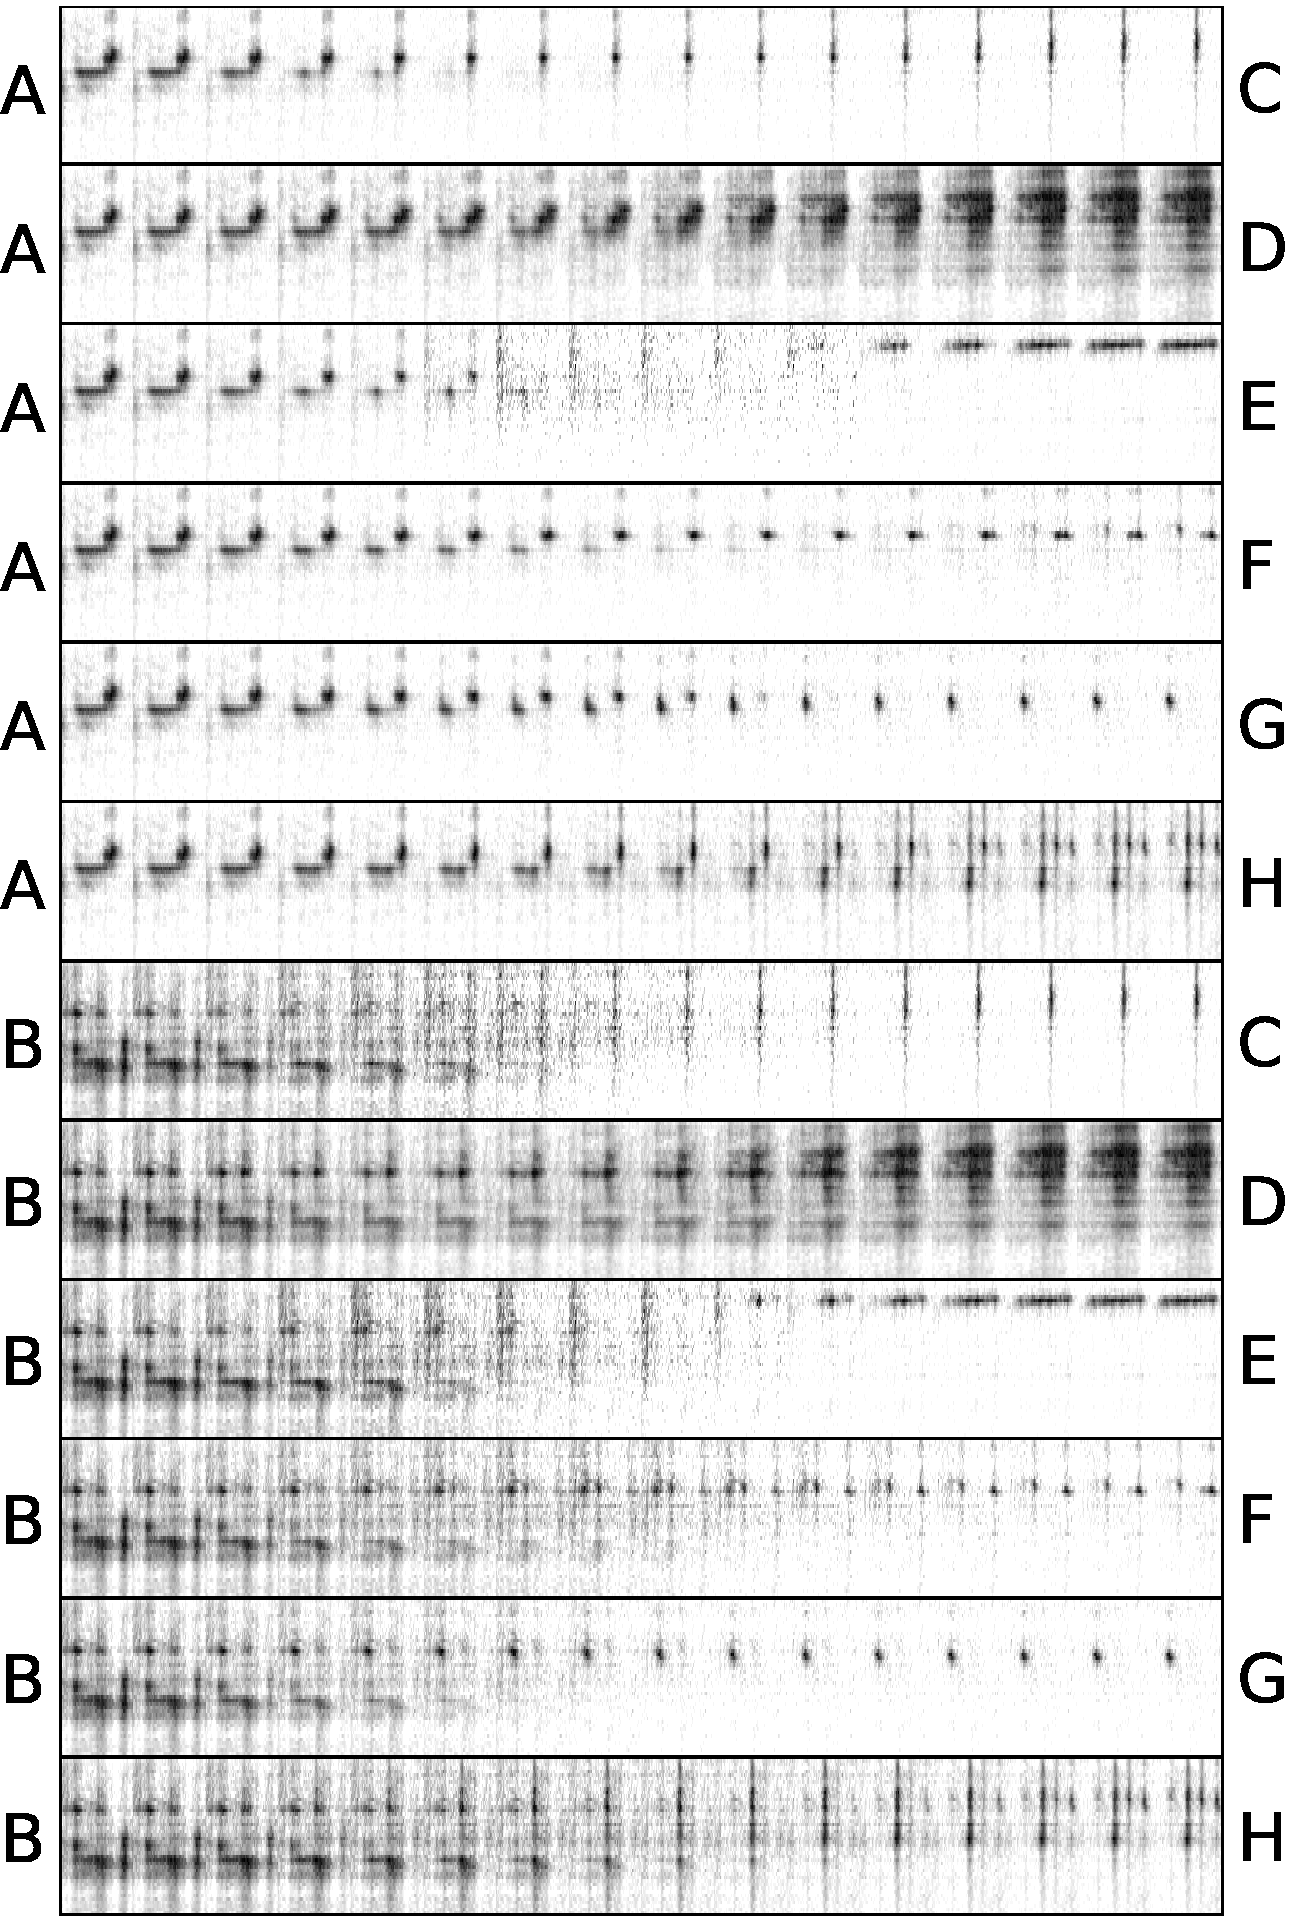
\includegraphics[height=.8\textheight]{figures/supplemental/sfig01a-all-morphs-1.pdf}
  \caption[Generated morph dimensions 1/2]
{12 example interpolated morph dimensions generated using the \DBN. 16 (of 128 used) example motifs for each morph dimension. Spectrogram representation with frequency on y-axis and time on the x-axis. Each motif is 400 ms long.
\index{morphs1}}
  \label{fig:morphs1}
\end{figure}
\begin{figure}[tbp] 
  \centering
  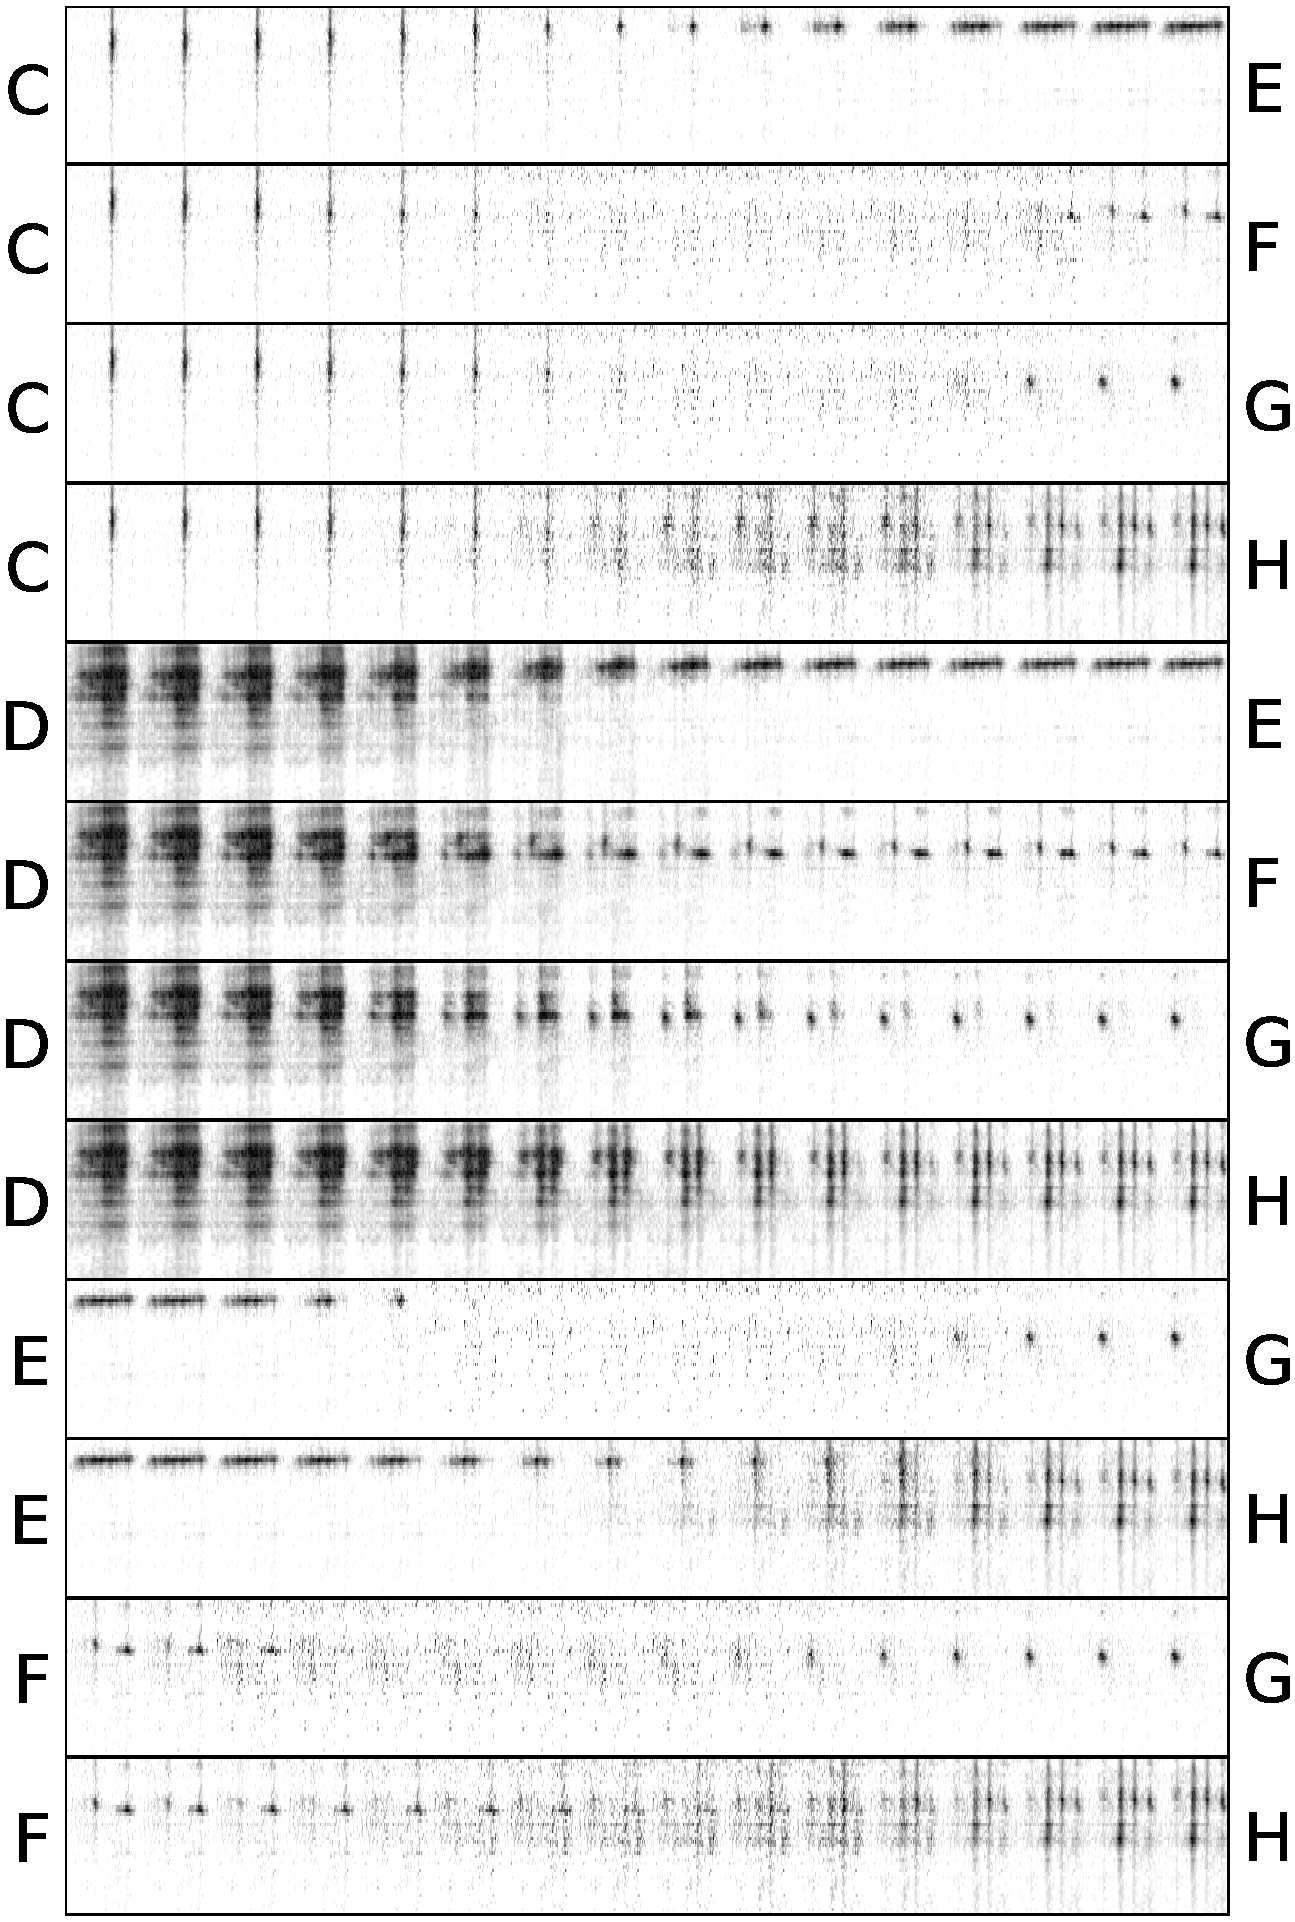
\includegraphics[height=.8\textheight]{figures/supplemental/sfig01b-all-morphs-2.pdf}
  \caption[Generated morph dimensions 2/2]
{12 example interpolated morph dimensions generated using the \DBN. 16 (of 128 used) example motifs for each morph dimension. Spectrogram representation with frequency on y-axis and time on the x-axis. Each motif is 400 ms long.
\index{morphs2}}
  \label{fig:morphs2}
\end{figure}
\begin{figure}[tbp] 
  \centering
  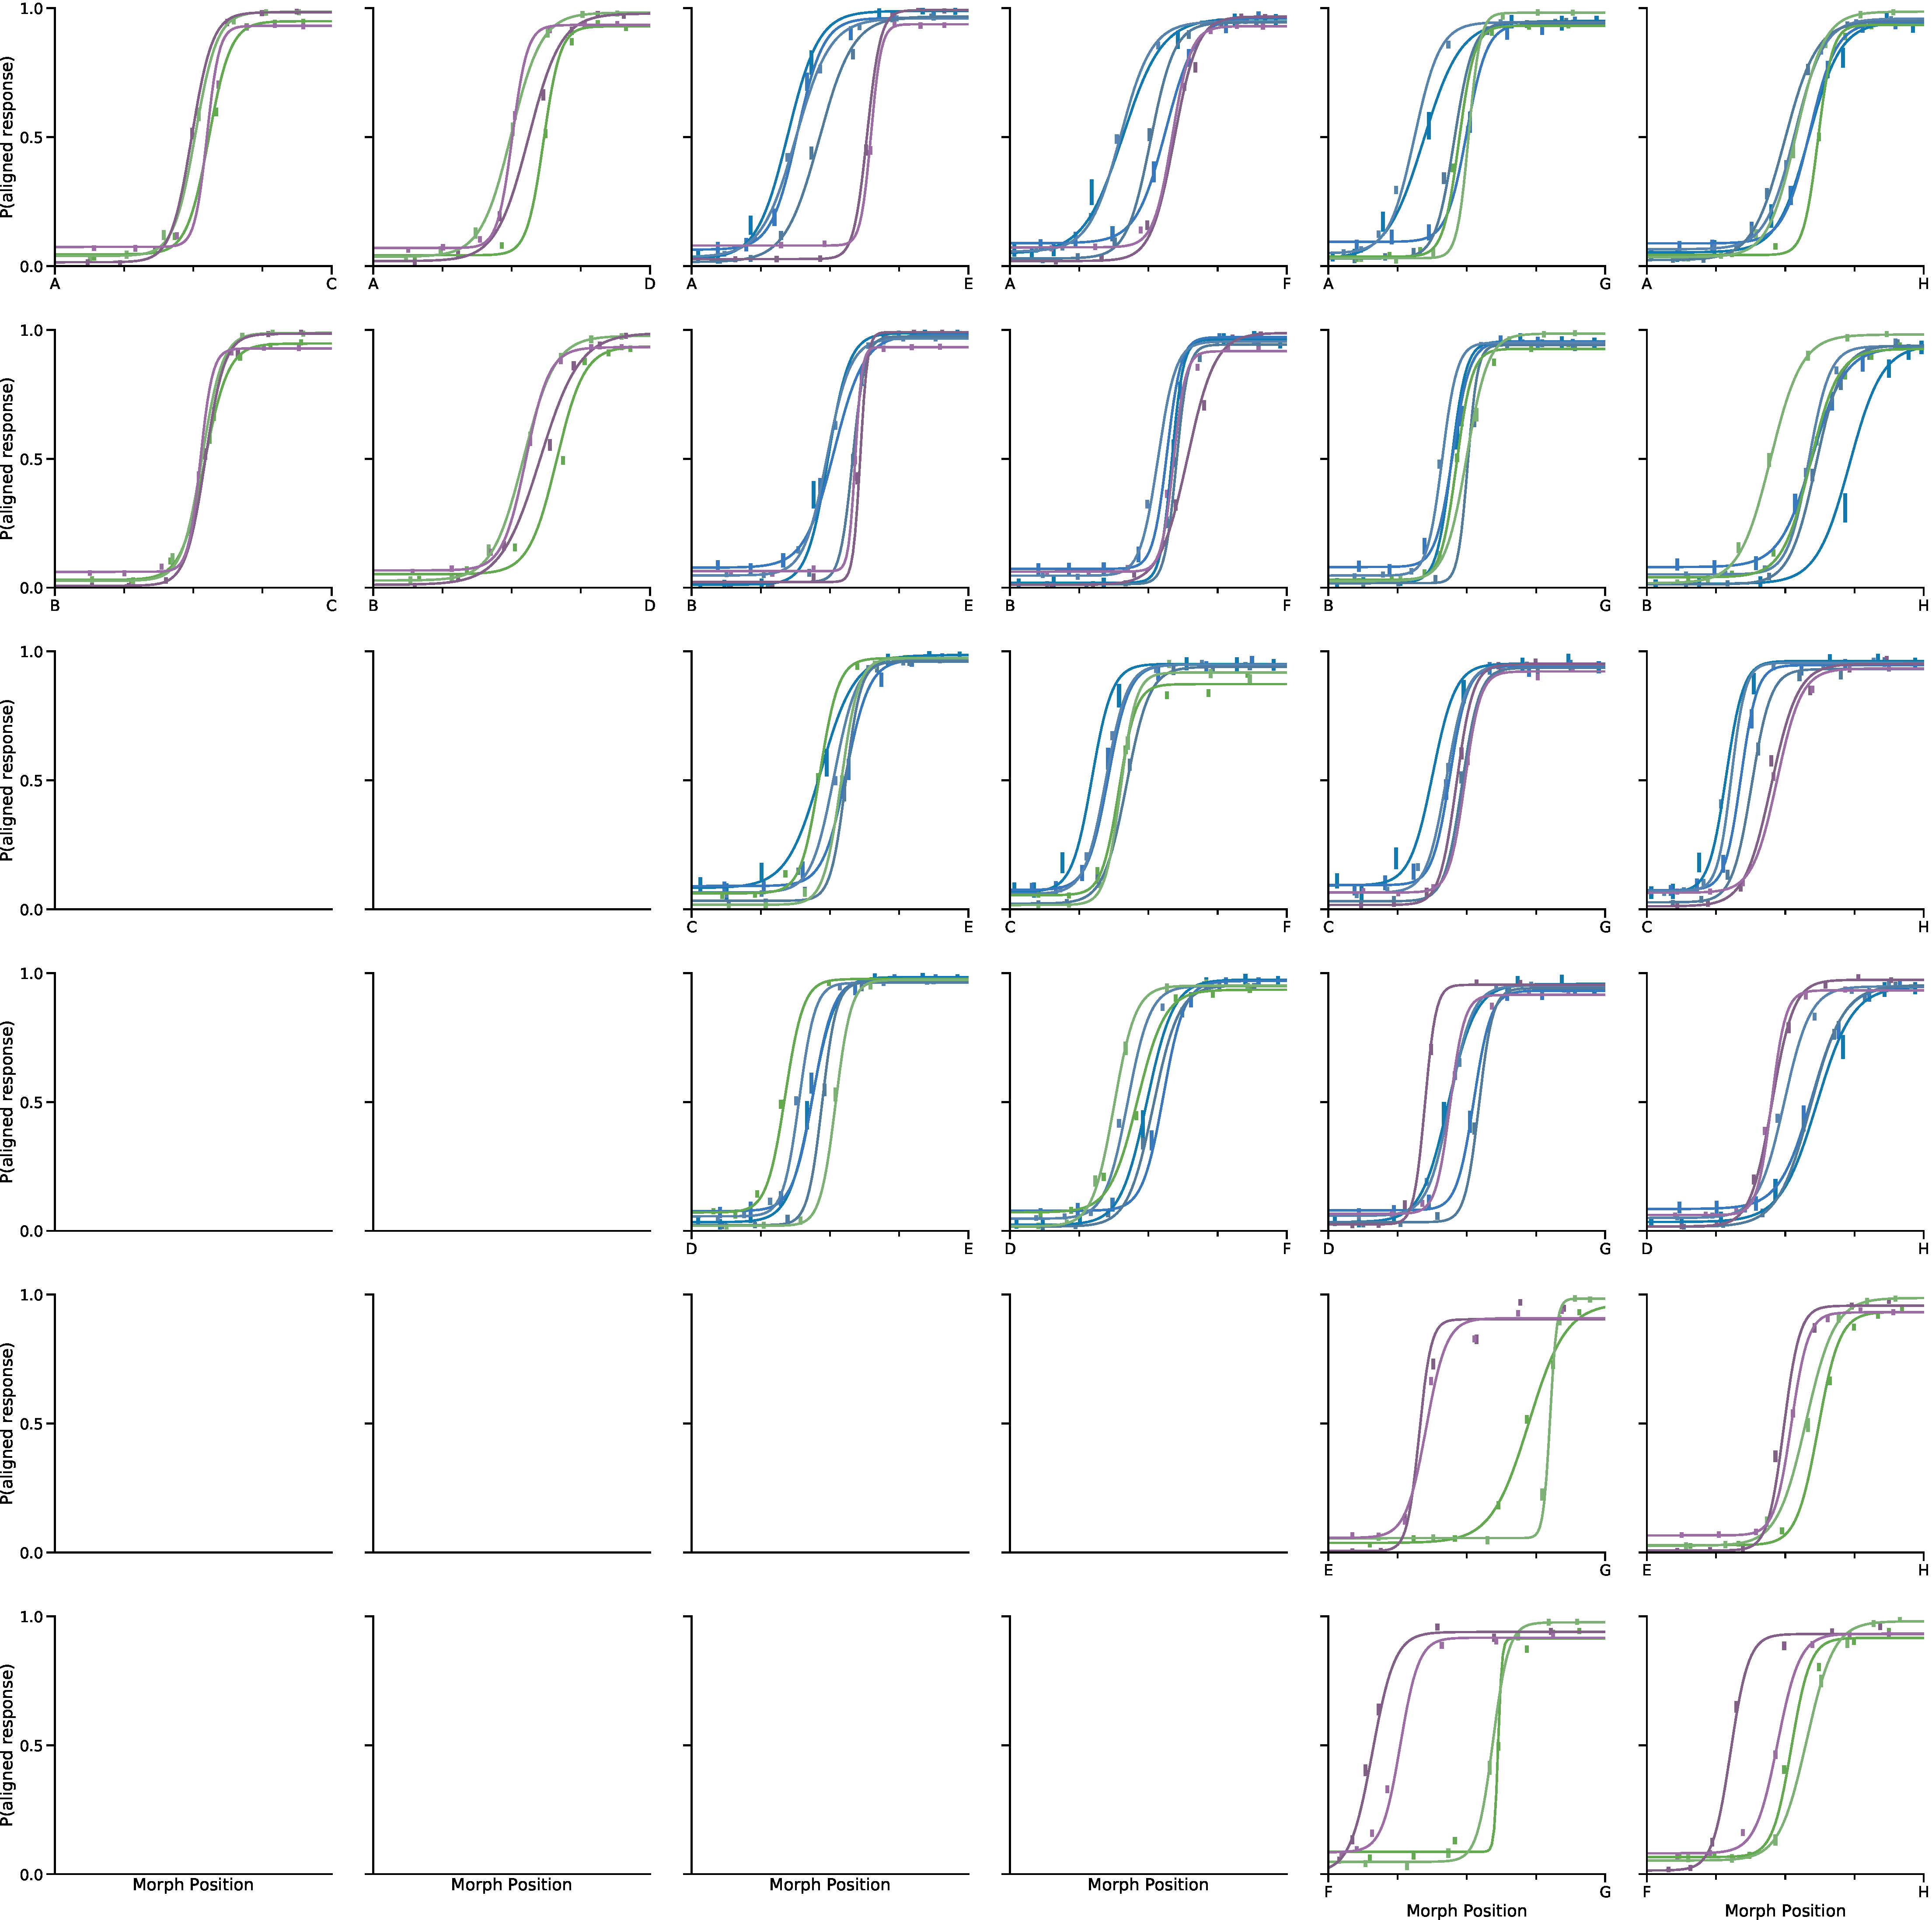
\includegraphics[width=174mm]{figures/supplemental/sfig02-psyc-all.pdf}
  \caption[All psychometric curves]
{Psychometric curves for all behavioral subjects on all 24 morph dimensions. Blue indicates the bird was part of cohort 1, purple, cohort 2, and green, cohort 3.
\index{psychometric-all}}
  \label{fig:psychometric-all}
\end{figure}
\begin{figure}[tbp] 
  \centering
  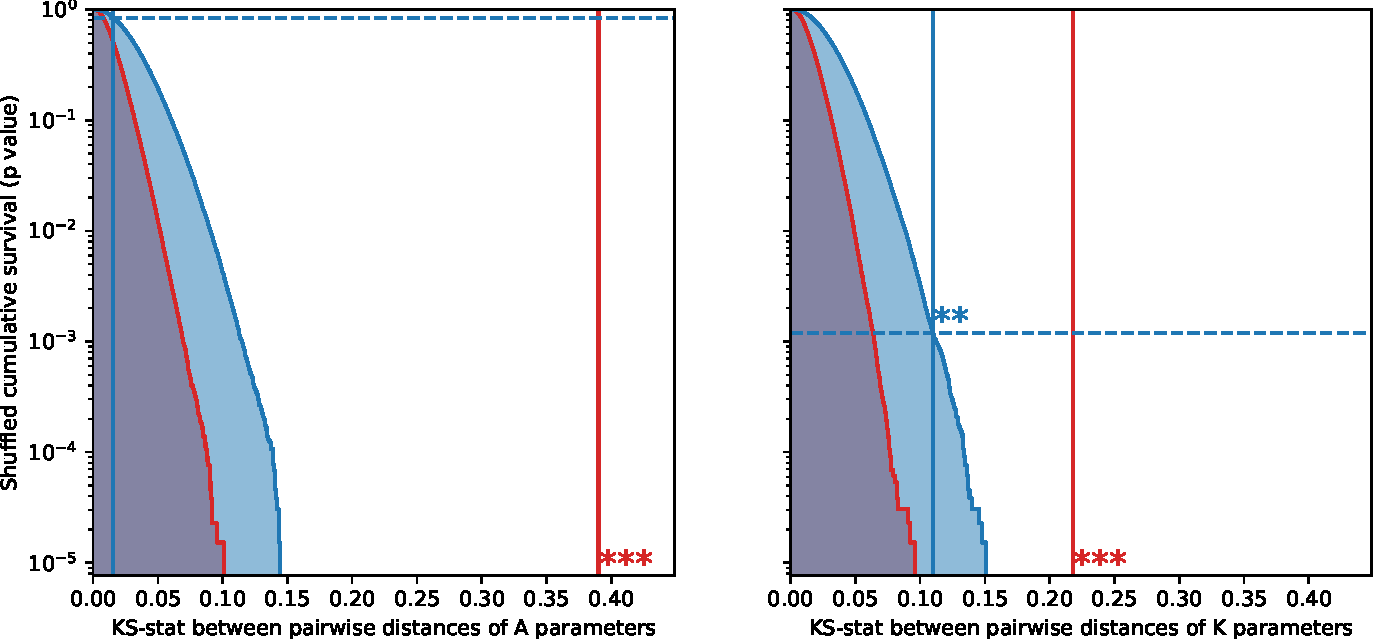
\includegraphics[width=174mm]{figures/supplemental/sfig03-psyc-conserved-stats-AK.pdf}
  \caption[Parameters A and K are conserved within subject.]
{The corresponding figure to \ref{fig:conserved}(E-F) for the scaling parameters A (left), and K (right).
\index{AKconserved}}
  \label{fig:AKconserved}
\end{figure}
\begin{figure}[tbp] 
  \centering
  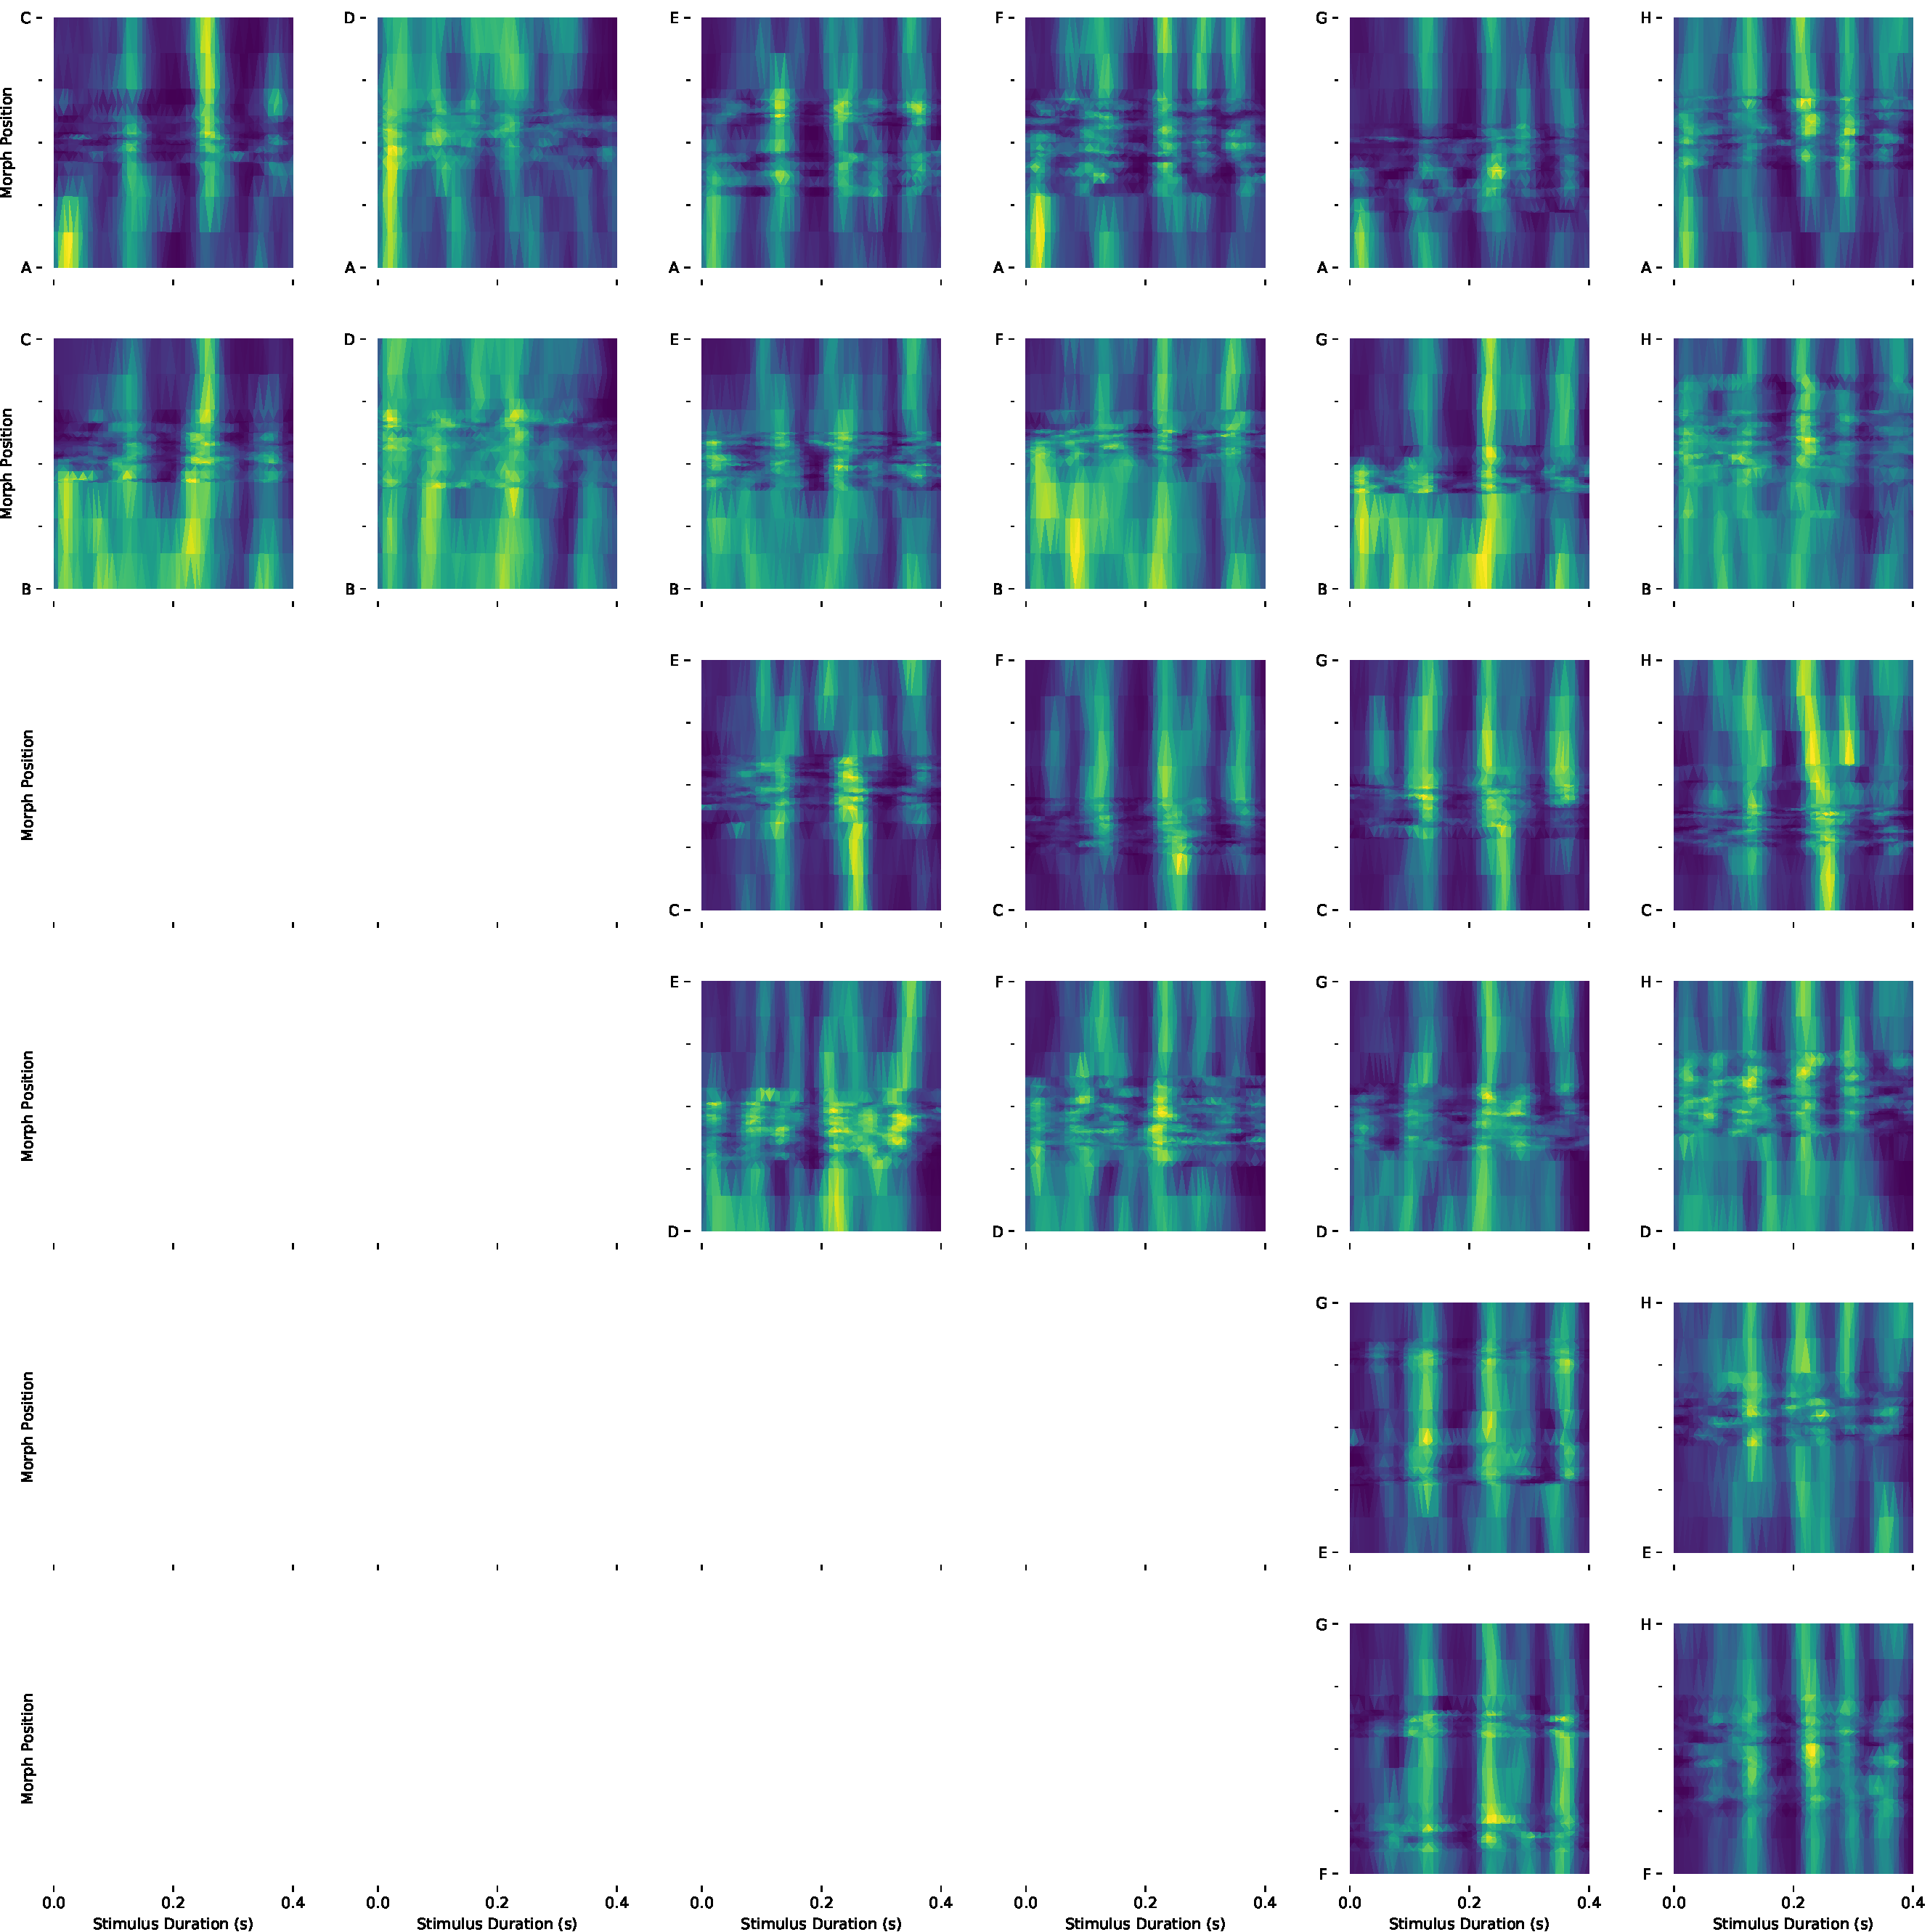
\includegraphics[width=\textwidth]{figures/supplemental/sfig04_morph_viz_all.pdf}
  \caption[Morph activity for 24 morph dimensions for a single neuron]
{Variation of the average Gaussian convolved single neuron’s representation across morph dimensions. Smoothly interpolated using triangulation for surface estimation. All 24 dimensions of the neuron plotted in figure \ref{fig:single} (F)
\index{single24}}
  \label{fig:single24}
\end{figure}
\begin{figure}[tbp] 
  \centering
  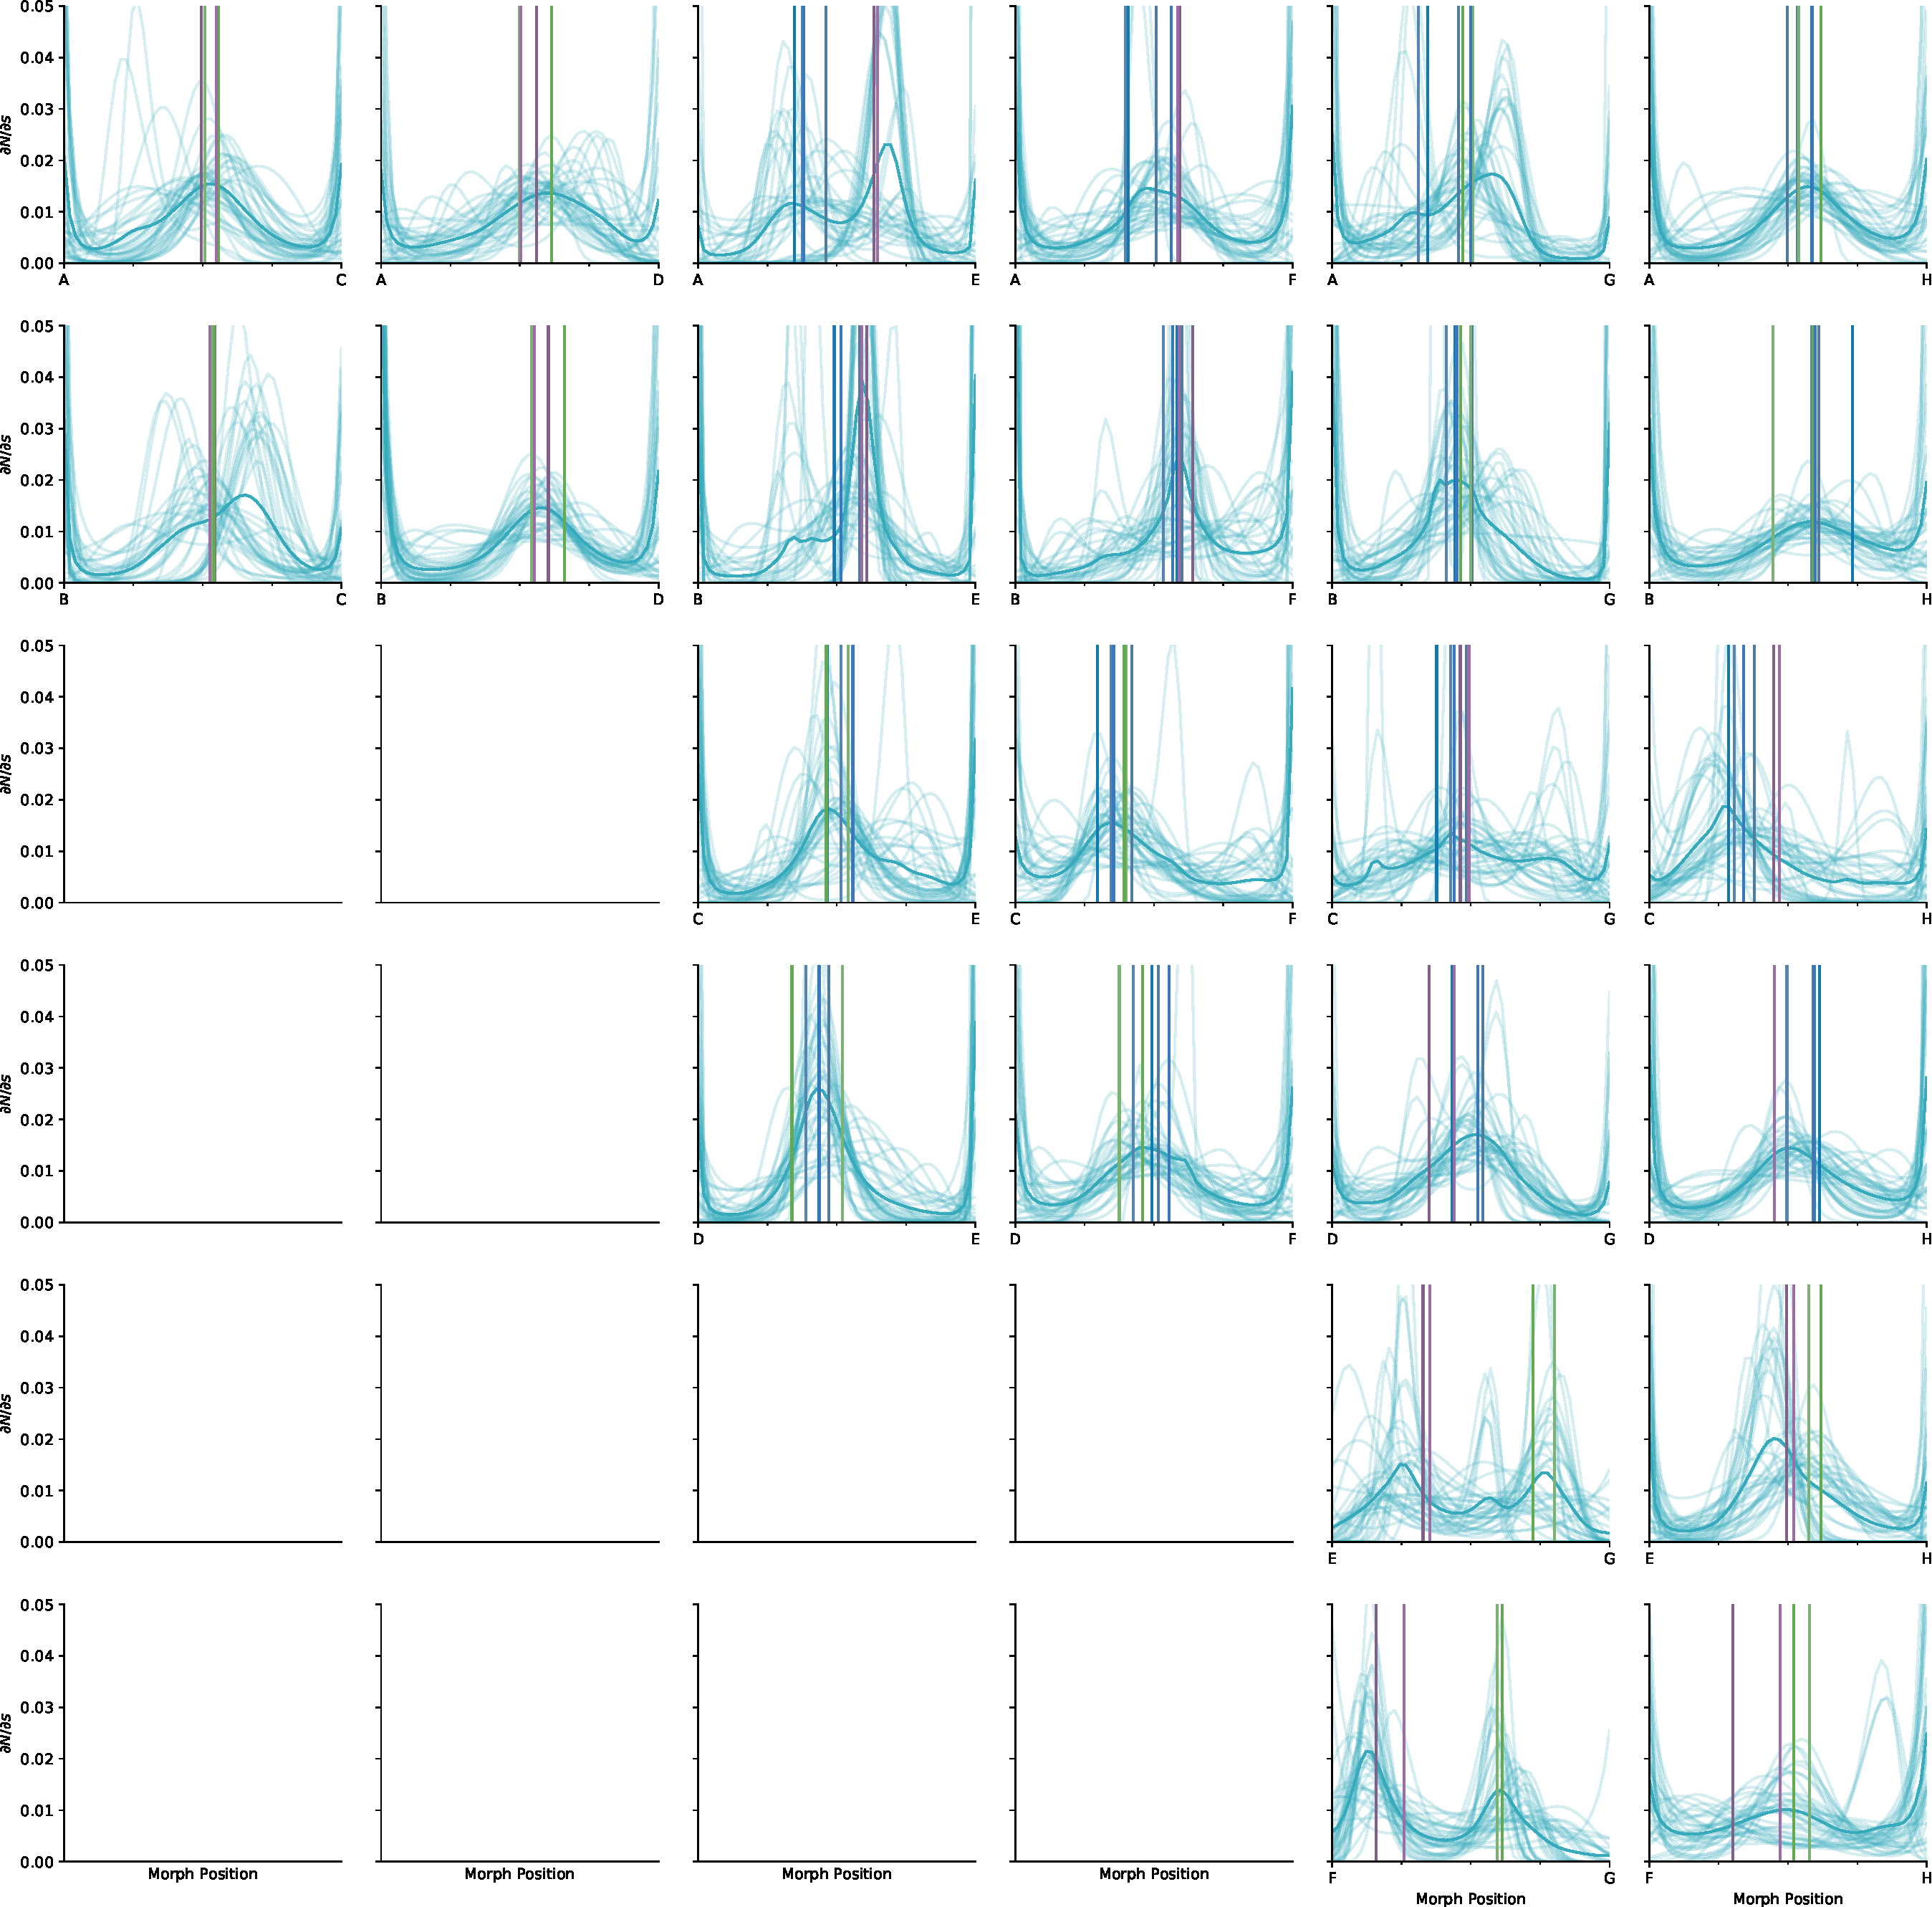
\includegraphics[width=\textwidth]{figures/supplemental/sfig05-thielk-4-all-morphs.pdf}
  \caption[4th order Thielk curves for all recorded populations on all 24 morph dimensions]
{4th order mean Thielk curves across all morph dimensions from all recorded neural populations. Corresponding to figure \ref{fig:derivative} (E-F).
\index{thielk-all}}
  \label{fig:thielk-all}
\end{figure}
\begin{figure}[tbp] 
  \centering
  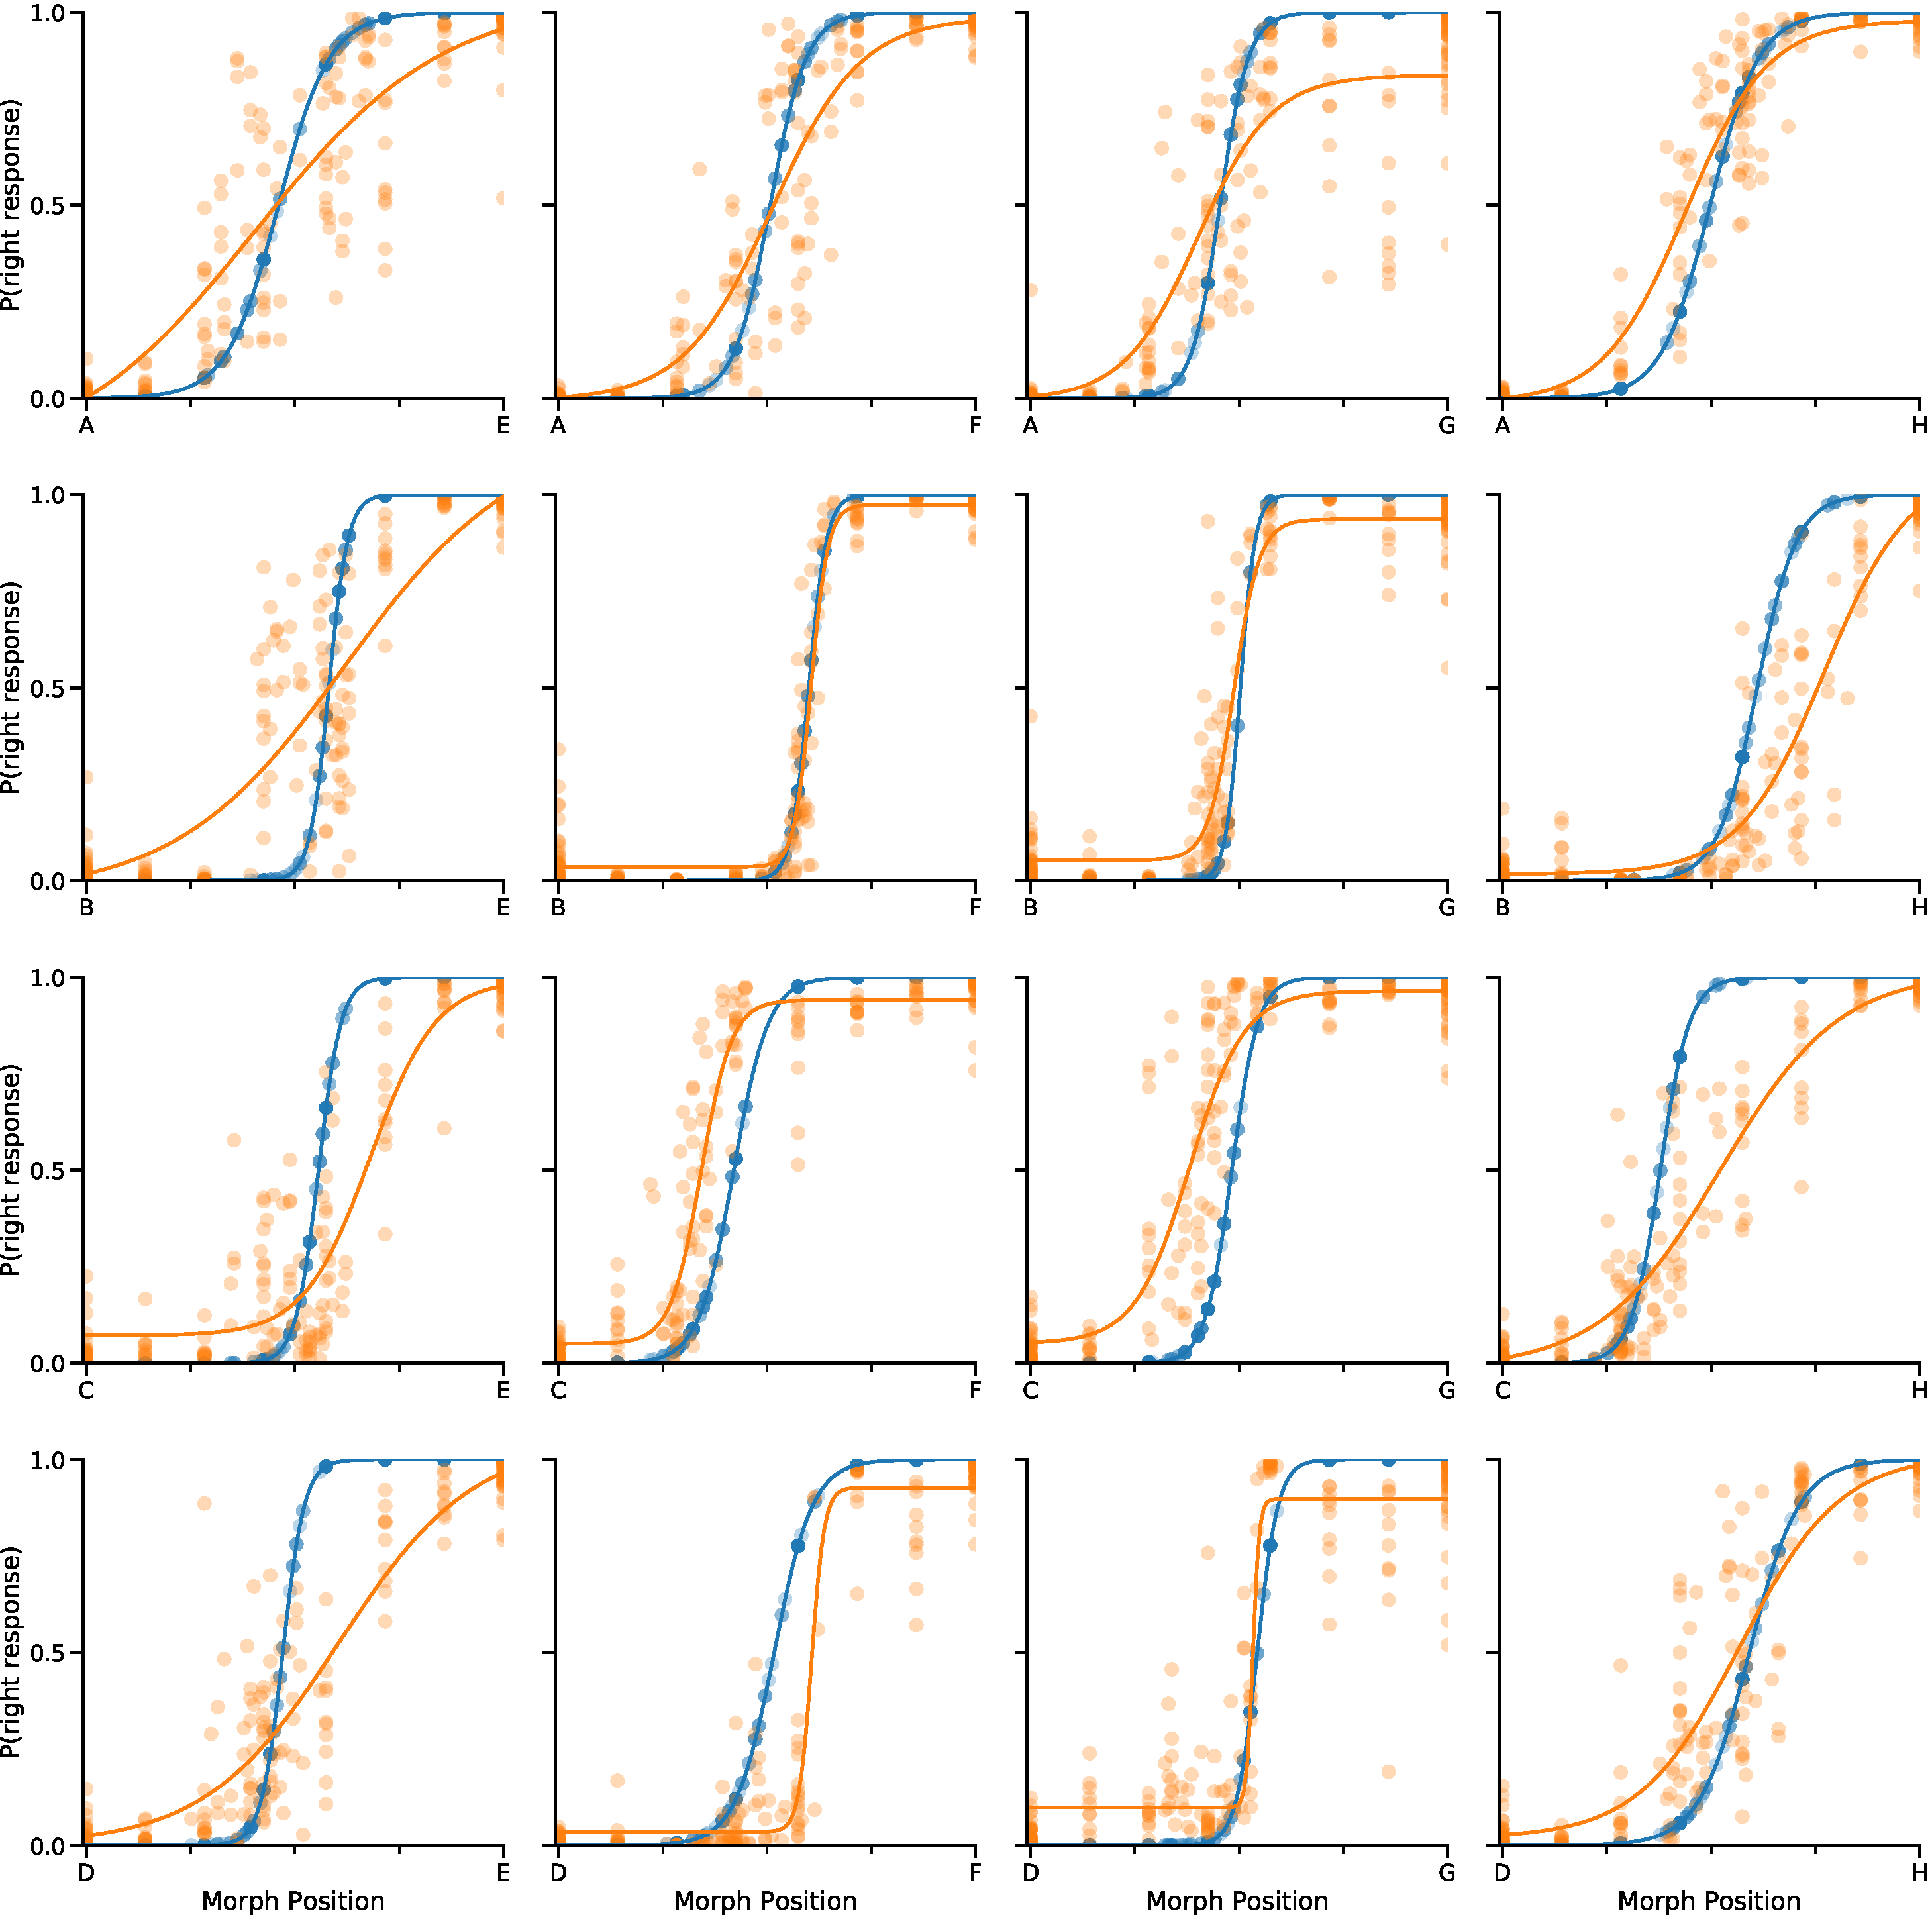
\includegraphics[width=\textwidth]{figures/supplemental/sfig06-neurometric-sample-all.pdf}
  \caption[All predicted Neurometric functions for a single population against a single behavioral subject]
{Predictions of behavioral psychometric curves for all morph dimensions for a single behavioral bird in cohort 1. Same neural population and behavioral bird as figure \ref{fig:neurometric} (A).
\index{neurometric-all}}
  \label{fig:neurometric-all}
\end{figure}
\renewcommand{\figurename}{Figure}
% \renewcommand{\thefigure}{\arabic{figure}}
\chapter{Predictive Coding}

\acf{PC} is the theory that the ``purpose'' of the perceptual system is not to encode the maximum amount of information about the current state of the world, but rather to provide a prediction of (the posterior distribution of) the future state of the world. 

Indeed, this provides a parsimonious explanation for much of the brain's function. If you consider a video of two people talking in a living room with an old TV displaying static - most of the Shannon information in the video will be in the TV's display. While the speck of static may be a result of a particle left by the big bang hitting the antenna, our brain doesn't devote the majority of its resources to keep track of the white noise patterns. i.e., the brain's sensory processing system isn't designed to maximize the mutual information between the sensory signals it receives. Instead, if you consider the temporal information, the brain tries to encode the predictive information within its sensory streams. \PC has been hailed by some as ``The unifying theory of the brain.''

\PC provided the inspiration and fundamental theory behind temporal difference learning, a class of model-free reinforcement learning methods which learn by bootstrapping from the current prediction of the state of the world. Temporal Difference Learning produced TD-Gammon, which was beating humans even before the more famous Deep Blue eventually beat Kasparov. Temporal Difference Learning is also one of the inspirations for many of the current state-of-the-art reinforcement learning applications such as AlphaGo by DeepMind and Five by OpenAI.

If we were prescribed to the theory of \PC we would expect that somewhere the brain has to encode 1) the prediction of what is to come, and 2) the error between the prediction and what came to pass. Indeed, some of the most famous work in neuroscience has demonstrated these values in predictions of reward in dopamine signaling in the VTA. However, the theory of \PC would expect that these values should exist throughout the perceptual system as well for all aspects of the state of the world. An excellent place to look for this would be where the brain processes complex time-varying signals, namely, in auditory processing regions.

A direct corollary of \PC is the notion of surprise which is a measure of how likely a stimuli is given its context. A simple formulation might be $\text{Surprise}=-\log P(S|C)$ where $S$ is the stimuli and $C$ is the context. Several normalizations or transformations have been applied to this formulation; however, this describes the fundamental idea. Some version of this formulation has been used to show that responses from secondary sensory regions are better described by models of surprise than by models using strictly the physical stimuli in both vision \cite{itti2005principled} and audition \cite{Gill2008}.

This formulation requires a model of the world that provides the predicted probability. Not too long ago, ``a model-free approach seems out of the question in the context of video processing, as it would take unreasonably too many data samples and hence unreasonably too long to accumulate sufficient data and allow accurate model-free estimation of the underlying probability density function (PDF) of the data'' \cite{itti2005principled}. However, this is no longer true with modern machine learning techniques and methods for handling significantly more data than was possible in 2005. Therefore I have spent some effort building some models that predict future posterior probability density function of spectrograms.

\section{Models}

\subsection{Deep mixture of beta distributions}
My first attempt was to create a neural network that, given a window of a spectrogram, predict the probability distribution of each frequency band in the next time bin of the spectrogram. The network was optimized by maximizing the log likelihood of the model. I modeled the probability distribution as a mixture of 3 beta distributions. The network was two fully connected layers with an output for a weight, $w$, and the two beta distribution parameters, $\alpha$ and $\beta$, for each of the three beta distributions, for each of the frequency bins. This network was very ill-behaved, and I spent considerable time implementing as many numerical analysis tricks to control and regularize the networks' exploding values. Most were relatively simple and included but was not limited to gradient clipping, different beta distribution approximations, the log-sum-exp trick and even an added cost function tied to the standard deviation of the beta distributions to try to prevent them from becoming delta functions.

One interesting method I used was adversarial training \cite{goodfellow2014explaining,lakshminarayanan2017simple}. Given an input $x$ with target $y$, and loss $l(\theta, x, y)$(e.g. $-\log p_\theta(y|x)$) \cite{goodfellow2014explaining} proposes the fast gradient sign method which generates an adversarial example as $x' = x + \epsilon \sign(\nabla_x l(\theta, x, y))$ and using $x'$ to augment the dataset by treating $(x', y)$ as an additional training example. Intuitively, this can be interpreted as a smoothing method by smoothing the likelihood around the target of an $\epsilon$-neighborhood around the training examples. This helped a small amount, but my networks still eventually got corrupted by NaNs. In my case where I'm predicting the likelihood of a full spectrogram slice, its possible adversarial training on my labels, $y$ might have also helped the stability. In the end, however, I began to strip away as many of the complexities of the network as I could to create a minimal viable network.

\subsection{Deep Gaussian prediction}
This minimum network was to simply predict each frequency band as a univariate Gaussian with a mean and a standard deviation, and let the network try and deal with any covariances. This network trained easily enough but didn't do nearly as good of a job at predicting as the deep mixture of beta distributions networks that were stopped before being corrupted by NaNs. However, even with this poor performance, I did notice peaks in the likelihood that corresponded to motif boundaries.

\subsection{Contrastive Predictive Coding}
The last method I have explored is \CPC\cite{CPC}. \CPC is a method that takes high dimensional time-varying data and attempts to do representation learning on it to provide a representation that captures the predictive information of the signal. They do this by encoding the high dimensional signal in a low dimensional latent space, $Z$, using an encoding network, and then feeding the latent space into a recurrent neural network which outputs a context in another latent space, $C$. $c_t$ is then used to linearly classify if a sample is actually the next time sample, or drawn from a distribution (I have used other random samples from the spectrogram). The whole model is learned end-to-end, providing an encoding network to a $Z$ space that both contains information that is useful for predictions, as well as information that is predictable. The model also provides the $C$ space, which also contains context from the past.

Figure \ref{fig:encoder} shows an example 8-dimensional $Z$ latent space learned by \CPC. It encodes all the predictive and predictable information contained in each spectrogram time slice. Noticeable changes in the spectrogram are reflected in some way in the encoded dimensions. It would be interesting to see if it allocated its weights in a similar distribution as would be predicted by the mel frequency scale.

\begin{figure}[tbp] 
  \centering
  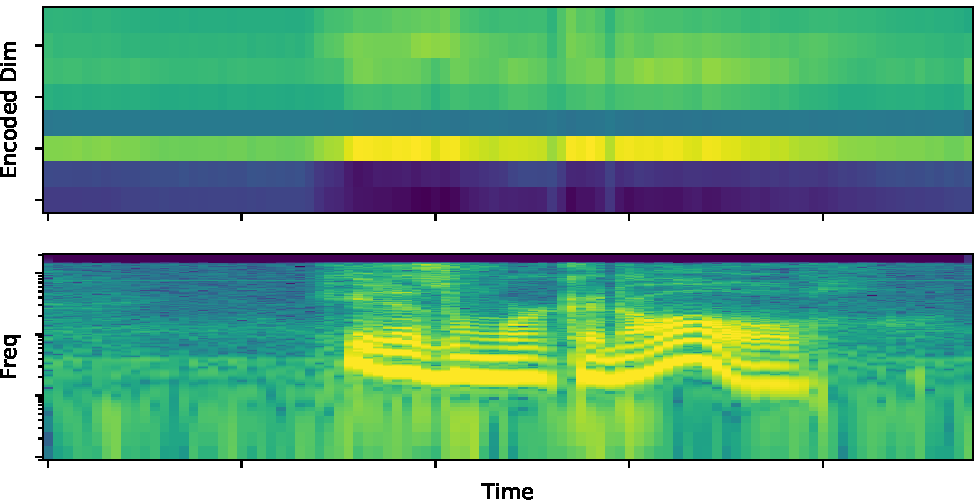
\includegraphics[width=\textwidth]{figures/encoder.pdf}
  \caption[8 dimensional $Z$ space learned by Contrastive Predictive Coding.]
{The representation learned by the encoder of \CPC. Top: The 8-dimensional latent space $Z$ created by pushing each 2048-dimensional spectrogram time slice through the encoder network. Bottom: 2048 Frequency bin spectrogram representation fed into the encoder and the \CPC network. The figure has been log scaled in the frequency axis to provide a visualization similar to a mel-scaled spectrogram; however, the 2048 dimensions are not log spaced so the \CPC network must learn where to allocate its weights to encode information in the predictive and predictable frequency dimensions. It would be interesting to see if the allocations it learns match that of a mel-scaled spectrogram.
\index{encoder}}
  \label{fig:encoder}
\end{figure}

\subsection{Future Improvements}
\CPC seems to be working quite well to generate representations, even though it doesn't give us explicit predictions. It would be possible to extract predictions from the \CPC network by 1) sampling from the latent space, or 2) explicitly using the linear decision boundary created by the network. There are also several other changes that could be made to the architecture which may improve the performance. A Wavenet \cite{van2016wavenet} style time dilation network architecture might allow for the removal of the LSTM or recurrent neural network and might improve training time. Alternatively, a transformer network \cite{vaswani2017attention} might be more efficient recurrent neural network architecture that is still able to capture the fundamental dynamics. Lastly, further skip-state predictions might improve the learned representations as hinted by \cite{gregor2018temporal}. There are many possible ways to incorporate skip state predictions into \CPC.

\section{Future Applications}

\subsection{Receptive Field Estimation}
These kinds of models have the potential to be used for much more than just posterior distribution prediction. As I alluded to in the introduction, an explicit model of the posterior distribution may allow for improved receptive field models and more accurate spike predictions. This would be done by splitting the stimuli explicitly into what was predicted, and how the actual stimuli differed from this prediction. Since the spiking could be dependent on the surprise at a variety of time lags, the dimensionality of this stimuli space quickly explodes as you consider farther back in time. To restrict the dimensions considered, a linear receptive field model should probably be used first to define the time lag limits and relevant frequency bands.

Alternatively, instead of using an explicit posterior prediction model, the learned \CPC encoded representation could be used to make spike predictions. This wouldn't require explicit arbitrary frequency limits which we have currently imposed by estimating the range of frequencies we believe the birds are sensitive to and by using a mel scale based on the human cochlear organization. Furthermore, by varying the dimensionality of the \CPC encoded representation, a balance between the encoded stimuli information and the limited experimental statistical power could be formed to combat the curse of dimensionality.

\subsection{Natural Unsupervised Segmentation of Vocal Objects}
Both word segmentation and motif segmentation has proven to be a non-trivial task and has limited efforts towards automatic vocal analysis. In both linguistics and birdsong research, hand segmentation remains the gold-standard technique for separating vocal objects. For human speech, some supervised methods do a reasonable job, mainly due to large amounts of labeled data. For birdsong, this is not available.

Preliminary data seems to indicate the usefulness of the likelihood of each time sample as an unsupervised segmentation signal. Previous methods at song segmentation in our lab mainly consisted of using the sum of the spectral power for each time point. I suspect that an improved method could use the likelihood of each time sample or its derivative. This makes intuitive sense because one would expect that intra-object predictability to be higher than inter-object predictability.

\subsection{General Encoding of High-dimensional Time-Varying Data}
Lastly, these techniques might be useful to extract meaningful information out of general high-dimensional time-varying data, of which we have a lot in Neuroscience. I suspect that the success of techniques like Independent Components Analysis (ICA) \cite{ICA}, Delay Differential Analysis \cite{DDA}, and Taken's delay embeddings indicate the kinds of statistical structure that are utilized by \CPC are abundant and informative in Neuroscience data. I expect this to be useful for many types of recordings including but not limited to EEG, fMRI, ECoG, LFP, and even recordings of many single units, mainly as an unsupervised dimensionality reduction technique.

%
% Of course, if you prefer, you can just start with
%   \chapter{My First Chapter Name}
% and start typing away.  

% \chapter{Just a Test}
% This is only a test.
% \section{A section}
% Lorem ipsum dolor sit amet, consectetuer adipiscing elit. Nulla odio
% sem, bibendum ut, aliquam ac, facilisis id, tellus. Nam posuere pede
% sit amet ipsum. Etiam dolor. In sodales eros quis pede.  Quisque sed
% nulla et ligula vulputate lacinia. In venenatis, ligula id semper
% feugiat, ligula odio adipiscing libero, eget mollis nunc erat id orci.
% Nullam ante dolor, rutrum eget, vestibulum euismod, pulvinar at, nibh.
% In sapien. Quisque ut arcu. Suspendisse potenti. Cras consequat cursus
% nulla.

% \subsection{A Figure Example}
% \label{ssec:figure_example}

% This subsection shows a sample figure.

% \begin{figure}[h] 
%   \centering
%   \includegraphics[width=0.5\textwidth]{sandiego}
%   \caption[A picture of San Diego. Short figure caption must be \protect{$< 4$} lines in the list of figures]
% {A picture of San Diego.  Short figure caption must be \protect{$< 4$} lines in the list of figures and match the start of the main figure caption verbatim. Note that figures must be on their own line (no neighboring text) and captions must be single-spaced and appear \protect\textit{below} the figure.  Captions can be as long as you want, but if they are longer than 4 lines in the list of figures, you must provide a short figure caption.\index{SanDiego}}
%   \label{fig:sandiego}
% \end{figure}

% \subsection{A Table Example}

% While in Section \ref{ssec:figure_example} Figure \ref{fig:sandiego} we had a majestic figure, here we provide a crazy table example.


% %%%% TABLE 1 %%%%
% \vspace{0.25in}
% \begin{table}[!ht]
% \caption[A table of when I get hungry.  Short table caption must be \protect{$< 4$} lines in the list of tables]{A table of when I get hungry. Short table caption must be \protect{$< 4$} lines in the list of tables and match the start of the main table caption verbatim.  Note that tables must be on their own line (no neighboring text) and captions must be single-spaced and appear \protect\textit{above} the table.  Captions can be as long as you want, but if they are longer than 4 lines in the list of figures, you must provide a short figure caption.}

% \vspace{-0.25in}
% \begin{center}
% \begin{tabular}{|p{1in}|p{2in}|p{3in}|}

% \hline
% Time of day & Hunger Level & Preferred Food \\

% \hline
% 8am & high & IHOP (French Toast) \\

% \hline
% noon & medium & Croutons (Tomato Basil Soup \& Granny Smith Chicken Salad) \\

% \hline
% 5pm & high & Bombay Coast (Saag Paneer) or Hi Thai (Pad See Ew) \\

% \hline
% 8pm & medium & Yogurt World (froyo!) \\

% \hline
% \end{tabular}
% \end{center}
% \label{tab:analysis3}
% \end{table}



%% APPENDIX
% \appendix
% \chapter{Final notes}
% What to do about things \cite{Martin_1983}.  What did he say \cite{Rilling_Insel_1999}.
%   Remove me in case of abdominal pain.



%% END MATTER
% \printindex %% Uncomment to display the index
% \nocite{}  %% Put any references that you want to include in the bib 
%               but haven't cited in the braces.
\bibliographystyle{apalike}  %% This is just my personal favorite style. 
%                              There are many others.
%\setlength{\bibleftmargin}{0.25in}  % indent each item
%\setlength{\bibindent}{-\bibleftmargin}  % unindent the first line
%\def\baselinestretch{1.0}  % force single spacing
%\setlength{\bibitemsep}{0.16in}  % add extra space between items
\bibliography{current}  %% This looks for the bibliography in template.bib 
%                          which should be formatted as a bibtex file.
%                          and needs to be separately compiled into a bbl file.
\end{document}

